%%%%%%%%%%%%%%%%%%% vorlage.tex %%%%%%%%%%%%%%%%%%%%%%%%%%%%%
%
% LaTeX-Vorlage zur Erstellung von Projekt-Dokumentationen 
% im Fachbereich Informatik der Hochschule Trier
%
% Basis: Vorlage svmono des Springer Verlags
%
%%%%%%%%%%%%%%%%%%%%%%%%%%%%%%%%%%%%%%%%%%%%%%%%%%%%%%%%%%%%%
\documentclass[envcountsame,envcountchap, deutsch]{i-studis}

\usepackage{makeidx}         	% Index
\usepackage{multicol}        	% Zweispaltiger Index
%\usepackage[bottom]{footmisc}	% Erzeugung von Fu�noten

%%-----------------------------------------------------
%\newif\ifpdf
%\ifx\pdfoutput\undefined
%\pdffalse
%\else
%\pdfoutput=1
%\pdftrue
%\fi
%%--------------------------------------------------------
%\ifpdf
\usepackage[pdftex]{graphicx}
\usepackage{epstopdf}
\usepackage[pdftex,plainpages=false]{hyperref}
%\else
%\usepackage{graphicx}
%\usepackage[plainpages=false]{hyperref}
%\fi

%%-----------------------------------------------------
\usepackage{color}				% Farbverwaltung
%\usepackage{ngerman} 			% Neue deutsche Rechtsschreibung
\usepackage[english, ngerman]{babel}
%\usepackage[latin1]{inputenc} 	% Ermöglicht Umlaute-Darstellung
\usepackage[utf8]{inputenc}  	% Ermöglicht Umlaute-Darstellung unter Linux (je nach verwendetem Format)

%-----------------------------------------------------
\usepackage{listings} 			% Code-Darstellung
\lstset
{
	basicstyle=\scriptsize, 	% print whole listing small
	keywordstyle=\color{blue}\bfseries,
								% underlined bold black keywords
	identifierstyle=, 			% nothing happens
	commentstyle=\color{red}, 	% white comments
	stringstyle=\ttfamily, 		% typewriter type for strings
	showstringspaces=false, 	% no special string spaces
	framexleftmargin=7mm, 
	tabsize=3,
	showtabs=false,
	frame=single, 
	rulesepcolor=\color{blue},
	numbers=left,
	linewidth=146mm,
	xleftmargin=8mm
}
\usepackage{textcomp} 			% Celsius-Darstellung
\usepackage{amssymb,amsfonts,amstext,amsmath}	% Mathematische Symbole
\usepackage[german, ruled, vlined]{algorithm2e}
\usepackage[a4paper]{geometry} % Andere Formatierung
\usepackage{bibgerm}
\usepackage{array}
\hyphenation{ Ele-men-tar-ob-jek-te  ab-ge-tas-tet Aus-wer-tung House-holder-Matrix Le-ast-Squa-res-Al-go-ri-th-men} 		% Weitere Silbentrennung bei Bedarf angeben
\setlength{\textheight}{1.1\textheight}
\pagestyle{myheadings} 			% Erzeugt selbstdefinierte Kopfzeile
\makeindex 						% Index-Erstellung

%--------------------------------------------------------------------------
\begin{document}
%------------------------- Titelblatt -------------------------------------
\title{Implementierung einer Enterprise Search Engine für das \\ Dietrich Online Projekt}
\subtitle{ Implementation of an enterprise search engine for the \\ Dietrich Online project }
%---- Die Art der Dokumentation kann hier ausgewählt werden---------------
%\project{Bachelor-Projektarbeit}
\project{Bachelor-Abschlussarbeit}
%\project{Master-Projektstudium}
%\project{Master-Abschlussarbeit}
%\project{Seminar zur Vorlesung ...}
%\project{Hausarbeit zur Vorlesung ...}
%--------------------------------------------------------------------------
\supervisor{Professor Doktor Christoph Schmitz} 		% Betreuer der Arbeit
\author{ Florian Reitz } 							% Autor der Arbeit
\address{Trier, den 15.10.2019} 							% Im Zusammenhang mit dem Datum wird hinter dem Ort ein Komma angegeben
\submitdate{15.3.2020} 				% Abgabedatum
%\begingroup
%  \renewcommand{\thepage}{title}
%  \mytitlepage
%  \newpage
%\endgroup
\begingroup
  \renewcommand{\thepage}{Titel}
  \mytitlepage
  \newpage
\endgroup
%--------------------------------------------------------------------------
\frontmatter 
%--------------------------------------------------------------------------
\preface

Diese Arbeit entstand als Abschlussarbeit an der Hochschule Trier in Zusammenarbeit mit der Bibliothek der Universität Trier. 
\newline
\newline
Die Idee zu dieser Arbeit entwickelte sich während meiner Arbeit am Dietrich online Projekt. Ich möchte diese Stelle nutzen, um mich beim Dietrich online Team und vor allem bei Herrn Kock für die Unterstützung zu bedanken.
\newline
\newline
Ein besonderer Dank gilt auch Herrn Professor Schmitz und Herrn Röpke für die Betreuung dieser Arbeit.
\newline
\newline
In dieser Arbeit wird aus Gründen der besseren Lesbarkeit das generische Maskulinum verwendet. Die dabei gewählte Form bezieht sich auf alle Geschlechter des Spektrums. 
\newline
Zudem wird DietrichOnline anstelle Dietrich online für eine bessere Lesbarkeit verwendet.
\newline
\newline
Der Code, der für diese Arbeit erstellt wurde, ist unter: \url{https://seafile.rlp.net/f/a70bebdfa575485a89ab/} zu finden. Das Passwort für den Download ist: Bachelor2020.
\newline
\newline
Trier, 2020
\newline
\noindent Florian Reitz				% Vorwort (optional)
\kurzfassung

%% deutsch
\paragraph*{German}
Diese Arbeit handelt von der Analyse diverser Enterprise-Suchmaschinen für das DietrichOnline-Projekt \ref{dietrichonline}. Dabei wurden die Suchmaschinen nach einer Anforderungsliste untersucht und die verbleibenden Kandidaten für einen Ersteindruck aufgesetzt. 

Nachdem sich für Elasticsearch entschieden wurde, wurde diese in einer Docker-Umgebung aufgesetzt. Dabei wurde auf eine verschlüsselte Kommunikation zwischen den einzelnen Systemen viel Wert gelegt.

Im letzten Teil der Arbeit wurde zudem eine prototypische Implementierung in das DietrichOnline-Projekt vorgenommen. Dafür wurde die Suche, sowie die Auto-Vervollständigung auf die Suchmaschine umgezogen.

%% englisch
\paragraph*{English}

This thesis analyzes various enterprise search-engines for the DietrichOnline project \ref{dietrichonline}. The search-engines were checked via a feature list and four of the remaining search engines were set up for a first impression.

After the decision was made for Elasticsearch, it was set up in a Docker environment. Great importance was attached to encrypted communication between the individual systems.

The last part of this thesis is a prototype implementation of the search engine in the DietrichOnline project. The search and the auto-completion function were set up to use Elasticsearch. 			% Kurzfassung Deutsch/English
\tableofcontents 						% Inhaltsverzeichnis
\listoffigures 							% Abbildungsverzeichnis (optional)
\listoftables 							% Tabellenverzeichnis (optional)
%--------------------------------------------------------------------------
\mainmatter                        		% Hauptteil (ab hier arab. Seitenzahlen)
%--------------------------------------------------------------------------
% Die Kapitel werden in separaten .tex-Dateien abgelegt und hier eingebunden.
\chapter{Einleitung und Problemstellung}

Begonnen werden soll mit einer Einleitung zum Thema, also Hintergrund und Ziel erl�utert werden.

Weiterhin wird das vorliegende Problem diskutiert: Was ist zu l�sen, warum ist es wichtig, dass man dieses Problem l�st und welche L�sungsans�tze gibt es bereits. Der Bezug auf vorhandene oder eben bisher fehlende L�sungen begr�ndet auch die Intention und Bedeutung dieser Arbeit. Dies k�nnen allgemeine Gesichtspunkte sein: Man liefert einen Beitrag f�r ein generelles Problem oder man hat eine spezielle Systemumgebung oder ein spezielles Produkt (z.B. in einem Unternehmen), woraus sich dieses noch zu l�sende Problem ergibt.

Im weiteren Verlauf wird die Problemstellung konkret dargestellt: Was ist spezifisch zu l�sen? Welche Randbedingungen sind gegeben und was ist die Zielsetzung? Letztere soll das
beschreiben, was man mit dieser Arbeit (mindestens) erreichen m�chte.
%\chapter{LaTeX-Bausteine}\label{Stile}

Der Text wird in bis zu drei Ebenen gegliedert:

\begin{enumerate}
  \item Kapitel ( \verb\chapter{Kapitel} ), \index{Kapitel}
  \item Unterkapitel  ( \verb \section{Abschnitt} ) und
  \item Unterunterkapitel  ( \verb \subsection{Unterabschnitte} ).
\end{enumerate}

\section{Abschnitt}\index{Abschnitt}
Text der Gliederungsebene 2.


\subsection{Unterabschnitt} \index{Unterabschnitt}
Text der Gliederungsebene 3.
Text Text Text Text Text Text Text Text Text Text Text Text Text Text Text
Beispiel für Quelltext \index{Quelltext} \\[2 ex]
\noindent
\begin{minipage}{1.0\textwidth} \small
\begin{lstlisting}
	Prozess 1:
	
	Acquire();
		a := 1;
	Release();
	...
	Acquire();
	if(b == 0)
	{					
		c := 3;
		d := a;
	}				
	Release();
\end{lstlisting}
\end{minipage}

\vspace{2cm}
\noindent
\begin{minipage}{1.0\textwidth} \small
\begin{lstlisting}
	Prozess 2:
	
	Acquire();
		b := 1;
	Release();
	...
	Acquire();
	if(a == 0)
	{					
		c := 5;
		d := b;
	}				
	Release();
\end{lstlisting}
\end{minipage}
\vskip 1em

Größere Code-Fragmente sollten im Anhang eingefügt werden.

\section{Abbildungen und Tabellen}

Abbildung\index{Abbildung} und Tabellen\index{Tabelle} werden zentriert eingefügt. Grundsätzlich sollen sie
erst dann erscheinen, nach dem sie im Text angesprochen wurden (siehe Abb. \ref{a1}). Abbildungen und Tabellen (siehe Tabelle \ref{t1}) können
im (fließenden) Text (\verb here ), am Seitenanfang (\verb top ), am Seitenende
(\verb bottom ) oder auch gesammelt auf einer nachfolgenden Seite (\verb page )
oder auch ganz am Ende der Ausarbeitung erscheinen. Letzteres sollte man nur
dann wählen, wenn die Bilder günstig zusammen zu betrachten sind und die
Ausarbeitung nicht zu lang ist ($< 20$ Seiten).

\begin{figure} %[hbtp]
	\centering
		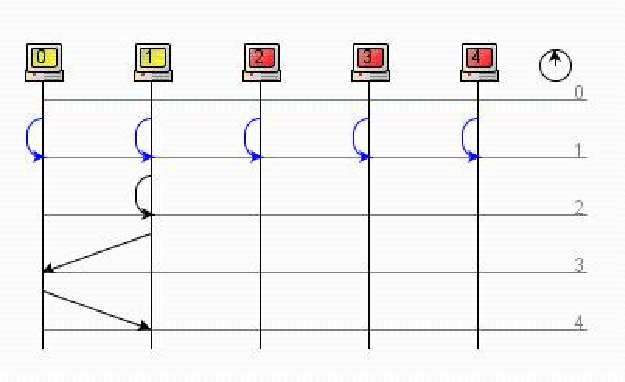
\includegraphics{images/p1ReadSeq.pdf}
	\caption{Bezeichnung der Abbildung}
	\label{a1}
\end{figure}

\begin{table} %[hbtp]
	\centering
		\begin{tabular}{l | l l l l}
		\textbf{Prozesse} & \textbf{Zeit} $\rightarrow$ \\
		\hline
			$P_{1}$ & $W(x)1$ \\
			$P_{2}$ & & $W(x)2$ \\
			$P_{3}$ & & $R(x)2$ & & $R(x)1$\\
			$P_{4}$ & & & $R(x)2$ & $R(x)1$\\
		\end{tabular}
	\caption{Bezeichnung der Tabelle}
	\label{t1}
\end{table}


\section{Mathematische Formel}\index{Formel}
Mathematische Formeln bzw. Formulierungen können sowohl im
laufenden Text (z.B. $y=x^2$) oder abgesetzt und zentriert im Text
erscheinen. Gleichungen sollten für Referenzierungen nummeriert
werden (siehe Formel \ref{gl-1}).
\begin{equation}
\label{gl-1}
e_{i}=\sum _{i=1}^{n}w_{i}x_{i}
\end{equation}

Entscheidungsformel:

\begin{equation}
\psi(t)=\left\{\begin{array}{ccc}
1 &  \qquad 0 <= t < \frac{1}{2} \\
-1 &  \qquad \frac{1}{2} <= t <1 \\
0 & \qquad sonst
\end{array} \right.
\end{equation}


Matrix:\index{Matrix}
\begin{equation}
A = \left(
\begin{array}{llll}
a_{11} & a_{12} & \ldots & a_{1n} \\
a_{21} & a_{22} & \ldots & a_{2n} \\
\vdots & \vdots & \ddots & \vdots \\
a_{n1} & a_{n2} & \ldots & a_{nn} \\
\end{array}
\right)
\end{equation}

Vektor:\index{Vektor} 

\begin{equation}
\overline{a} = \left(
\begin{array}{c}
a_{1}\\
a_{2}\\
\vdots\\
a_{n}\\
\end{array}
\right)
\end{equation}

\section{Sätze, Lemmas und Definitionen}\index{Satz}\index{Lemma}\index{Definition}

Sätze, Lemmas, Definitionen, Beweise,\index{Beweis} Beispiele\index{Beispiel} können in speziell dafür vorgesehenen Umgebungen erstellt werden.

\begin{definition}(Optimierungsproblem)

Ein \emph{Optimierungsproblem} $\mathcal{P}$ ist festgelegt durch ein Tupel
$(I_\mathcal{P}, sol_\mathcal{P}, m_\mathcal{P}, goal)$ wobei gilt

\begin{enumerate}
\item $I_\mathcal{P}$ ist die Menge der Instanzen,
\item $sol_\mathcal{P} : I_\mathcal{P} \longmapsto \mathbb{P}(S_\mathcal{P})$ ist eine Funktion, die jeder Instanz $x \in I_\mathcal{P}$ eine Menge zulässiger Lösungen zuweist,
\item $m_\mathcal{P} : I_\mathcal{P} \times S_\mathcal{P} \longmapsto \mathbb{N}$ ist eine Funktion, die jedem Paar $(x,y(x))$ mit $x \in I_\mathcal{P}$ und $y(x) \in sol_\mathcal{P}(x)$ eine
Zahl $m_\mathcal{P}(x,y(x)) \in \mathbb{N}$ zuordnet (= Maß für die Lösung $y(x)$ der Instanz $x$), und
\item $goal \in \{min,max\}$.
\end{enumerate}

\end{definition}

\begin{example} MINIMUM TRAVELING SALESMAN (MIN-TSP)
\begin{itemize}
\item $I_{MIN-TSP} =_{def}$ s.o., ebenso $S_{MIN-TSP}$
\item $sol_{MIN-TSP}(m,D) =_{def} S_{MIN-TSP} \cap \mathbb{N}^m$ 
\item $m_{MIN-TSP}((m,D),(c_1, \ldots , c_m)) =_{def} \sum_{i=1}^{m-1} D(c_i, c_{i+1}) + D(c_m,c_1)$ 
\item $goal_{MIN-TSP} =_{def} min$
\end{itemize}
\begin{flushright}
$\qed$
\end{flushright}
\end{example}

\begin{theorem} Sei $\mathcal{P}$ ein \textbf{NP}-hartes Optimierungsproblem.
Wenn $\mathcal{P} \in$ \textbf{PO}, dann ist \textbf{P} = \textbf{NP}.
\end{theorem}

\begin{proof} Um zu zeigen, dass \textbf{P} = \textbf{NP} gilt, genügt es
wegen Satz A.30 zu zeigen, dass ein einziges \textbf{NP}-vollständiges
Problem in \textbf{P} liegt. Sei also $\mathcal{P}'$ ein beliebiges \textbf{NP}-vollständiges Problem.

Weil $\mathcal{P}$ nach Voraussetzung \textbf{NP}-hart ist, gilt insbesondere
$\mathcal{P}' \leq_T \mathcal{P}_C$. Sei $R$ der zugehörige
Polynomialzeit-Algorithmus dieser Turing-Reduktion.
Weiter ist $\mathcal{P} \in$ \textbf{PO} vorausgesetzt, etwa vermöge eines
Polynomialzeit-Algorithmus $A$. Aus den beiden
Polynomialzeit-Algorithmen $R$ und $A$ erhält man nun
leicht einen effizienten Algorithmus für $\mathcal{P}'$: Ersetzt man
in $R$ das Orakel durch $A$, ergibt dies insgesamt eine polynomielle
Laufzeit. 
%\begin{flushright}
$\qed$
% \end{flushright}
\end{proof}

\begin{lemma} Aus \textbf{PO} $=$ \textbf{NPO} folgt \textbf{P} $=$ \textbf{NP}.
\end{lemma}

\begin{proof} Es genügt zu zeigen, dass unter der angegeben
Voraussetzung KNAPSACK $\in$ \textbf{P} ist.

Nach Voraussetung ist MAXIMUM KNAPSACK $\in$ \textbf{PO},
d.h. die Berechnung von $m^*(x)$ für jede Instanz $x$ ist
in Polynomialzeit möglich. Um KNAPSACK bei Eingabe
$(x,k)$ zu entscheiden, müssen wir nur noch $m^*(x) \geq k$
prüfen. Ist das der Fall, geben wir $1$, sonst $0$ aus. Dies
bleibt insgesamt ein Polynomialzeit-Algorithmus. 
\begin{flushright}
$\qed$
\end{flushright}
\end{proof}

\section{Fußnoten}

In einer Fußnote können ergänzende Informationen\footnote{Informationen die für die Arbeit zweitrangig sind, jedoch für den Leser interessant sein könnten.} angegeben werden. Außerdem kann eine Fußnote auch Links enthalten. Wird in der Arbeit eine Software (zum Beispiel Java-API\footnote{\url{http://java.sun.com/}}) eingesetzt, so kann die Quelle, die diese Software zur Verfügung stellt in der Fußnote angegeben werden.

\section{Literaturverweise}\index{Literatur}
Alle benutzte Literatur wird im Literaturverzeichnis angegeben\footnote{Dazu wird ein sogennanter bib-File, literatur.bib verwendet.}. Alle angegebene Literatur sollte mindestens einmal im Text referenziert werden.
\chapter{Dietrich-Online Projekt}
\label{dietrichonline}

TODO!
\chapter{Vergleich der Enterprise Search Engines}

In ersten Schritt werden diverse Enterprise Search Engines evaluiert. Dafür wurde eine Anforderungsliste mit den Mitarbeitern erstellt. Die Systeme welche bei diesen Vergleich nach Features am besten abschneiden werden anschließend aufgesetzt, getestet und genauer verglichen.

\begin{itemize}
    \item Open Source oder Kostenlos
    \item Unterstützung von Facetten
    \item Ranking der Suchergebnisse
    \item Volltextsuche
    \item Support für PDF, SQL, XML
    \item Logging-Möglichkeit
\end{itemize}

Des Weiteren sind die folgenden Funktionen auch wichtig, allerdings keine K.O. Kriterien:

\begin{itemize}
    \item Support für PostgreSQL
    \item Backup Funktionen
    \item Auto-Korrektur und Auto-Vervollständigung
    \item Security Features
    \item PHP-Support
    \item bezahlter Support
\end{itemize}

Durch die begrenzten finanziellen Mittel und die lange Projektlaufzeit besteht die Notwendigkeit eine kostenfreie, im besten Fall sogar Open Source Suchmaschine zu finden. Auch äußerst wichtig ist der Support für Facetten, da viele Dietrich-Online als Suchmaschine den Nutzer einige Tools zum Verfeinern seiner Suchergebnisse zur Verfügung stellen will. Das Ranking der Suchergebnisse ist vor allem für die Transparenz wichtig, da hier mit vielen Daten gearbeitet wird, welche allerdings nicht alle gleichzeitig dargestellt werden können. Dieses Problem kann mit einer Gewichtung der Suchergebnisse behoben werden, welches dann auf der Seite für Transparenz veröffentlicht wird. Die Volltextsuche wird es möglich machen auch nach Schlüsselwörtern im Titel zu suchen. Der Support von den verschiedenen Dateiformaten ergibt sich dadurch, dass dieses Projekt stark gewachsen ist. Es gibt viele Prozessschritte, welche auf denselben Daten in verschiedenen Formen arbeiten. Darunter werden alle Einträge im XML Format bearbeitet, es gibt alle Scans als PDF und für die Webseite sind alle Daten nochmals in der Datenbank vorhanden. Dadurch gibt sich auch das Problem, dass Daten mehrfach vorliegen welches sicherlich Später von größerer Bedeutung sein wird. Als letztes ist es noch wichtig, dass eine Logging-Möglichkeit geboten wird, damit schnell und effizient Probleme mit dem System erkannt und gelöst werden können.

Ein Support für PostgreSQL ist für dieses Projekt nicht so wichtig, allerdings könnte es sein, dass der Server später auch andere Datenbanken verwaltet. Der Server wird sowieso täglich durch einen Automatismus gesichert. Allerdings ist eine manuelle Backup-Lösung wünschenswert, um die Suchmaschine losgelöst von den Server zu sichern und gegebenenfalls auch einfach auf einen anderen Server umzuziehen. Auto-Korrektur und Auto-Vervollständigung sind beide sehr interessant, um den Nutzer mehr Komfort-Funktionen bieten zu können. Der Server sollte ja generell nur intern Ansprechbar sein. Allerdings gibt es für manche der Suchmaschinen eine Web-Oberfläche, da wäre es wichtig eine sichere Verbindung dorthin und gegebenenfalls eine Möglichkeit der Mehrfaktor-Authentifizierung zu haben. Einen PHP-Connector, welcher Objekte zum Umgang mit der Suchmaschine bietet, wäre wünschenswert. Allerdings bieten einige Suchmaschinen auch die Möglichkeit über JSON Anfragen an die Suchmaschine zu stellen. Allerdings sollte zumindest eine der beiden Möglichkeiten gegeben sein. Zuletzt wäre für akute Probleme ein bezahlter Support, der dafür schneller reagiert wünschenswert. 

\section{Apache Lucene Core}
\label{lucenecore}

Lucene Core ist eine Open Source Enterprise Search Engine von der Apache Foundation geschrieben in Java.

Das Lucene Projekt wurde im Jahre 1997 vom Entwickler Doug Cutting gestartet. 2001 ist es dann der Apache Foundation als Teil des Jakarta-Projekts beigetreten und wurde 2005 ein eigenes Hauptprojekt der Foundation. \cite{Wikipedia.2019c}

Lucene Core erfüllt alle der Grundanforderungen. Für das Monitoring gibt es eine Klasse, die es auch ermöglicht, dass langsame Query’s geloggt werden. Zudem bietet es Support für PostgreSQL und Auto-Korrektur/Auto-Vervollständigung. Da es keine Web-Oberfläche besitzt, gibt es auch keine weiteren Sicherheitsfunktionen. Einen PHP-Connector gibt es leider auch nicht, man müsste daher mit PHP direkte Systemaufrufe an Java machen. Bezahlten Support gibt es hier nicht, da dieses Projekt zur Apache Foundation gehört. 
\cite{TheApacheSoftwareFoundation.2019b}

\section{Terrier}
\label{terrier}

Terrier ist eine Open Source Enterprise Search Engine geschrieben in Java. Entwickelt und gepflegt wird diese von der University of Glasgow. Sie existiert bereit seit 10 Jahren und besitzt, laut Webseite, eine breite Nutzerbasis. 
Terrier erfüllt leider nicht alle Grundanforderungen, da es keine direkte Möglichkeit gibt SQL zu indexieren. Es gibt allerdings eine Möglichkeit das SQL in JSON zu konvertieren und dieses dann in die Suchmaschine einzupflegen. Auch scheint es kein Support für Facetten gegeben.
\cite{McCreadie.2019}

\section{Sphinx}
\label{sphinx}

Sphinx ist eine Suchmaschine entwickelt von Andrew Aksyonoff. Das Akronym steht für „SQL Phrase Index“.\cite{SphinxTechnologiesInc.b} Bis zur Version 2 wurde sie aktiv Open Source entwickelt. Ab Version 3 wurde die Entwicklung closed Source. Auf der Github-Seite steht: „The sources for 3.0 will also be posted here when we decide to make those publicly available.“ \cite{sphinxserach.2019}, also gibt es kein genaues Datum ob und wann die Version 3 Open Source geht. Version 3.1.1 wurde im Oktober 2018 veröffentlicht und seitdem lässt sich auch nichts mehr über das Projekt finden. Von daher ist davon auszugehen, dass das Projekt nicht mehr weitergeführt wird. 

Zu den Features ist festzuhalten, dass es keinen nativen PDF-Support in der Open-Source Version existiert, ab der Version 3 jedoch wurde ein Dokumenten-Speicher eingebaut. Allerdings werden die anderen Anforderungen alle erfüllt. Es existiert, laut Webseite, sogar ein bezahlter Support, allerdings ist fraglich, ob man mit der Firma noch in Kontakt treten kann. \cite{SphinxTechnologiesInc.2019}

\section{Apache Solr}
\label{solr}

Apache Solr ist eine, auf Lucene Core \ref{lucenecore} viel eingesetzte Search Engine von der Apache Foundation. Sie basiert auf Apache Lucene Core und erweitert dieses um ein grafische Benutzeroberfläche und einige Features. 
Die Entwicklung dafür begann 2004 als ein internes Projekt von CNET um eine bessere Suche für die eigene Webseite zu bieten. Später im Jahre 2006 hat CNET dann den Source Code an die Apache Foundation weitergegeben. Dadurch wurde  es zu einem eigenen Projekt bei der Apache Foundation. Im Jahre 2009 wurden Solr dann in das Apache Lucene Projekt eingefügt. Dort wird es auch aktuell noch weiterentwickelt. \cite{Wikipedia.2019b}

Solr wird unter anderem von DuckDuckGo und Best Buy eingesetzt. Durch die Unterstützung von der Apache Foundation längerfristige Weiterentwicklung abzusehen. 

Da Solr zur Apache Foundation gehört, ist es Open Source. Es bietet viele Funktionen von Haus, damit erfüllt es alle Grundanforderungen und besitzt darüber hinaus auch Support für fast alle Bonus-Features. Einzig und allein gibt es keinen bezahlten Support, dafür allerdings eine große Community, welche man durch einen Mailing Liste oder IRC erreichen kann.

\cite{TheApacheSoftwareFoundation.2019}

\section{ElasticSearch}
\label{elasticsearch}

Eine weitere großes Enterprise Search Engine ist ElasticSearch. Auch dieses Projekt arbeitet auf der Basis von Lucene. Zu den bekanntesten Kunden zählen Ebay und Adobe. Gestartet wurde das Projekt in den jungen 2000ern von Shay Banon, um eine Verwaltung für die Rezepte seiner Frau zu schaffen. Im Juni 2012 haben sich dann Logstash, ein Logging Dienst, Kibana, ein UI für ElasticSearch, und ElasticSearch zusammengetan. Alle kamen zusammen in der ElasticSearch Incorporated. Seitdem wurden der Produktkatalog stetig erweitert und die Produkte weiterentwickelt. Viele der weiteren Produkte sind allerdings nicht mehr Open-Source oder kostenlos. Der ELK-Stack ist allerdings weiterhin kostenlos und ElasticSearch zudem auch als Open-Source Variante zu haben. Eine genauere Aussage, welche Features nur in der kostenlosen und nicht in der Open-Source Variante zu finden sind, finden sich in der Tabelle \ref{vglTable}.

ElasticSearch erfüllt alle der Grundanforderungen, auch in der Open-Source Variante. Auch viele der optionalen Features kann man in der Open Source Variante genießen. Einzig die Sicherheitsfunktionen, wie rollen-basierte Authentifizierung sind der kostenlosen Variante vorbehalten. Eine Möglichkeit auf bezahlten Support besteht auch, dafür muss auf eine bezahlte Version gewechselt werden, was auch einige Funktionen wie IP-Filter mit sich bringt. Allerdings ist diese daraufhin auch nichtmehr Open-Source. \cite{Elasticsearch.2019}

\section{Fess}
\label{fess}

Fess ist eine Enterprise Search Engine basierend auf ElasticSearch entwickelt von dem japanischen Unternehmen CodeLibs. Die Suchmaschine ist komplett Open-Source und wird unter der Apache-Lizenz entwickelt.

Die Suchmaschine erfüllt alle Grundanforderungen. Darüber hinaus bietet es Support für PostgreSQL, Backups (sogar über die Web-Oberfläche) und Auto-Korrektur und Vervollständigung. Es gibt keinen direkten PHP Support, allerdings können anfragen über JSON geschickt werden. Ein bezahlter Support ist auch möglich über die Firma N2SM Incorporated. \cite{N2SM.2019} Bei dieser Arbeiten anscheinend auch einige der Entwickler von FESS. Sicherheitsfunktionen werden über rollen-basierte Authentifizierung mitgeliefert. \cite{CodeLibs.2019}

\section{Algolia}
\label{algolia}

Algolia ist eine cloud-basierte Search Engine, welche unter anderem von Twitch und Lacoste verwendet wird. Die Suchmaschine wird hierbei als SAAS (Software as a Service) angeboten.  Hierbei lädt man die Daten auf Algolia Server und dann daraufhin der API Suchen auf den Daten ausführen.

Es erfüllt alle Grundanforderungen, wobei allerdings in der kostenlosen Variante grade einmal 10 Tausend Einträge und 50 Tausend Operationen im Monat erlaubt sind. Diese Einschränkung macht die kostenlose Variante dieser Suchmaschine für das Dietrich-Online Projekt unbrauchbar. Von den optionalen Anforderungen erfüllt Algolia auch alle. Der bezahlte Support wird ab der Starter Edition für 30 Dollar im Monat mitgeliefert. \cite{Algolia.2019}

\section{Manticore Search}
\label{manticore}

Manticore Search Engine ist eine Open-Source Solution basierend auf Sphinx \ref{sphinx}. Nachdem Sphinx Closed-Source gegangen ist, wurde auf der letzten offenen Version die erste Version von Manticore Search entwickelt. Zu den großen Kunden zählen unter anderem Craigslist und Boardreader.

Manticore erfüllt fast alle Grund Anforderungen, allerdings ist kein nativer PDF-Support gegeben. Es muss daher auf eine Konvertierung der Daten auf XML gesetzt werden. Es findet sich außerdem eine Unterstützung von PostgreSQL, sowie Auto-Korrektur und Vervollständigung. Es gibt auch einen Query-Log. Zuletzt gibt es noch eine Option auf bezahlten Support. Die Supportkosten sind dabei direkt auf der Webseite angegeben und belaufen sich auf 3000 Dollar im Jahr für den Standard Support. \cite{ManticoreSoftwareLtd.2019}

\section{Xapian}
\label{xapian}

Xapian ist eine Open-Source Enterprise Suchmaschine, welche von Zeit-Online, der Universitätsbibliothek Köln und der Debian Webseite genutzt wird. Die Suchmaschine basiert auf Open Muscat, einer Suchmaschine, welche an der Cambridge Universität in den 1980ern von Dr. Martin Porter entwickelt wurde. In 2001, als Open Muscat Closed-Source ging, haben sich einige Entwickler die letzte offene Version geladen und diese weiterentwickelt.

Sie erfüllt alle der Grundanforderungen, wenn auch Logging nur im Grundsinne erfüllt wird, da nur Errors geschmissen werden. Des Weiteren bietet die Suchmaschine Support für PostgreSQL. Auch eine Replikations-Funktion wird mitgeliefert. Sie bietet auch Auto-Korrektur und Auto-Vervollständigung. Ein Login-System mit Sicherheitsfunktionen gibt es durch das Fehlende Frontend Administration nicht. Es gibt allerdings die Möglichkeit mit Omega eine CGI-Suche zu nutzen. Diese Suche bietet allerdings keine Administration, sondern nur eine grafische Oberfläche für Suchanfragen.

Auch gibt es eine Möglichkeit für bezahlten Support. Auf der Webseite werden zwei Firmen angegeben, welche bezahlten Support bieten. Allerdings funktioniert der Link aktuell nur für eine der beiden Firmen aktuell. Zudem ist ein PHP-Connector für die Suchmaschine vorhanden, was die Einbindung ist das Projekt vereinfacht. \cite{XAP.2019}

\section {Vorauswahl}

Alle Suchmaschinen die zumindest die Grundanforderungen erfüllen, werden hier in der Tabelle nun nochmals aufgeführt für einen leichteren Vergleich. 

\begin{table} %[hbtp]
	\centering
		\begin{tabular}{l | l | l | l | l | l | l | l}
		& \textbf{LC} & \textbf{SH} & \textbf{AS} & \textbf{ES}  & \textbf{FE} & \textbf{AG} & \textbf{XP} \\
        \hline
        Open Source oder Kostenlos                  & x & x  & x & x  & x & x  & x  \\
        Unterstützung von Facetten                  & x & x  & x & x  & x & x  & x  \\
        Ranking der Suchergebnisse                  & x & x  & x & x  & x & x  & x  \\
        Volltextsuche                               & x & x  & x & x  & x & x  & x  \\
        Support für PDF, SQL, XML                   & x & x* & x & x  & x & x  & x  \\
        Monitoring / Logging                        & x & x  & x & x  & x & x  & x? \\
        \hline
        Support für PostgreSQL                      & x & x  & x  & x  & x & x  & x \\
        Backup                                      & - & -  & x  & x  & x & x+ & - \\
        Auto-Korrektur und Vervollständigung        & x & x  & x  & x  & x & x  & x \\
        Security Features                           & - & -  & x- & x* & x & x  & - \\
        PHP Support                                 & - & x  & x  & x  & - & x  & x \\
        bezahlter Support                           & - & x  & -  & x  & x & x  & x \\
        \hline
        unter aktiver Entwicklung**                 & x & -  & x  & x  & x & x  & x \\
        offizelles Docker Image                     & - & -  & x  & x  & x & -  & - \\
        Synonym Support                             & x & x  & x  & x  & x & x  & x \\
        Web-Interface                               & - & -  & x  & x  & x & x  & - \\
        Plugin Support                              & - & x  & x  & x  & x & -  & - \\
        JSON oder RESTful API                       & - & x* & x  & x  & x & -  & x-- \\
        SQL-Like Query Support                      & - & x  & x  & x  & - & -  & - \\
		\end{tabular}
    \caption{Feature-Vergleich der verschiedenen Enterprise Suchmaschinen }
    \label{vglTable}

    *  = Feature nur in der kostenlosen Variante verfügbar. \\
    ** = Update innerhalb des letzen halben Jahres \\
    -- = Nur mit Omega CGI installiert \\
    +  = Anbieter kümmert sich um das Feature \\
    -  = Funktion nur per Plugin Implementiert \\

    Die Tabelle vergleicht einige Features der ausgewählten Search Engines. Dabei wurden die Namen aus Platzgründen wie folgt abgekürzt:

    \begin{itemize}
        \item LC = Lucene Core \ref{lucenecore}
        \item SH = Sphinx \ref{sphinx}
        \item AS = Apache Solr \ref{solr}
        \item ES = ElasticSearch \ref{elasticsearch}
        \item FE = Fess \ref{fess}
        \item AG = Algolia \ref{algolia}
        \item XP = Xapian \ref{xapian}
    \end{itemize} 


\end{table}


Nach einem ersten Überblick wurden nun Aufgrund der Auswahlkriterien diese Systeme zum genaueren Vergleich ausgewählt: Apache Solr, Manticore Search, ElasticSearch (in der kostenlosen Version) und Xapian. Lucene Core wird nicht genauer untersucht, da Solr ein umfassenderes Paket bietet, welches den gestellten Anforderungen mehr entspricht.
\chapter{Genauer Vergleich}

In diesem Kapitel werden die vorher ausgewählten Suchmaschinen genauer verglichen. Dafür werden alle vier Suchmaschinen aufgesetzt und getestet. Hier wird Wert auf alle Aspekte des Prozesses gesetzt. Da ich dieses Projekt nicht nach meiner Bachelor-Arbeit wohl nicht weiter verfolgen kann, ist es auch wichtig zu schauen, wie leicht ein neuer Administrator sich in das System einlernen kann, beziehungsweise wie leicht das System zu verstehen und administrieren ist. Deshalb wird auch die Dokumentation verglichen und geschaut, wie groß die Community der einzelnen Suchmaschinen ist. Die genaueren Kriterien werden nun im Folgenden mit Erkärungen aufgeführt.

Das Test-System hat folgende Spezifikationen:

\begin{itemize}
    \item CPU: 4 Kerne
    \item RAM: 16 Gigabyte
    \item Festplattenspeicher: 500 GB
    \item Betriebssystem: Ubuntu
\end{itemize} 

Auf das System wird daraufhin die MySQL Datenbank von Dietrich-Online Projekt aufgespielt. Dies für diesen Vergleich die einzige Datenquelle sein.

\section{Aufbau der Tests}

\subsection{Installation}

Im ersten Schritt wird die Installation bewertet, dabei wird geschaut, wie einfach es ist die Software zu installieren. Hierbei ist es wichtig zu schauen, wie simpel die Installation ist. Existiert zum Beispiel ein Installations-Wizard? Wie viel muss manuell in den Dateien geändert werden? Müssen viel externe Programme nachinstalliert werden?

\subsection{Oberfläche}

Als Nächstes folgt der Ersteindruck der Software und Oberfläche. Dabei wird geschaut, wie übersichtlich die Oberfläche ist, falls eine gegeben ist, und wie verständlich das System für Einsteiger ist. Dafür wird im ersten Schritt möglichst auf die Dokumentation verzichtet, um einen Ersteindruck zu liefern, wie gut die Oberfläche für sich selbst spricht. Dies dient dazu um, zu schauen wie der neue Administrator bestimmte Aufgaben ohne Vorkenntnisse erfüllen kann. Besondere Punkte dabei sind zum Beispiel: Wie viel kann man über die Oberfläche konfigurieren? Lassen sich Updates direkt über die Oberfläche einspielen? Ist die Seite responsive? Wie funktioniert die Nutzerverwaltung?

\subsection{Indexierung}

Hier geht es darum festzustellen, wie einfach eine Indexierung der einzelnen Dateien möglich ist. Darunter fällt zum Beispiel: Kann man die Daten über die grafische Benutzeroberfläche indexieren lassen? Kann man das System darauf anweisen Änderungen direkt neu zu indexieren?


\subsection{Dokumentation}

Im dritten Schritt wird die Dokumentation analysiert. Hierbei wird das Augenmerk auf die Übersichtlichkeit und Verständlichkeit gelegt. Auch hier ist es wieder wichtig zu schauen, ob die Dokumentation auch ohne Vorkenntnisse gut zu verstehen ist. Da in diesen Kurztest nicht alle Funktionen durchgetestet werden können, ist es leider auch nicht möglich zu schauen, ob alle Funktionen korrekt und ausführlich dokumentiert sind. Sollte allerdings schon von den Grundfunktionen eine schlechte oder fehlende Dokumentation auffallen wird dies natürlich erwähnt. 

\subsection{Datenschutz}

Hier geht es darum zu schauen, ob das Tool nach Hause telefoniert. Dann soll noch überprüft werden, ob die Logdateien anonymisiert und nach gewisser Zeit gelöscht werden können.

\subsection{Absetzen einer Anfrage und Integration in PHP}

Im letzten Schritt werden einige Query’s abgesetzt. Dies wird zum einen über die Oberfläche geschehen, falls vorhanden, und was wichtiger ist über die Schnittstelle für PHP. Dafür wird ein PHP-Script geschrieben und die Laufzeit des Scripts gemessen.

Der erste Query ist einer der am aktuell am langsamsten läuft. Er ermittelt alle Lemmata vom Buchstaben S und baut alle Daten, die zur Anzeige benötigt werden zusammen \ref{img:errorListSample}. Die Tabellen die für diese Ansicht gebraucht werden, sind in diesen Diagramm \ref{img:lAdminStructure} zu finden. Eigentlich muss man sagen, dass es sich hierbei nicht um einen Query handelt, sondern um zwei. Der erste Sammelt alle ID’s aus der Datenbank, welche unter dem Buchstaben zu finden sind:

\begin{figure}
	\centering
	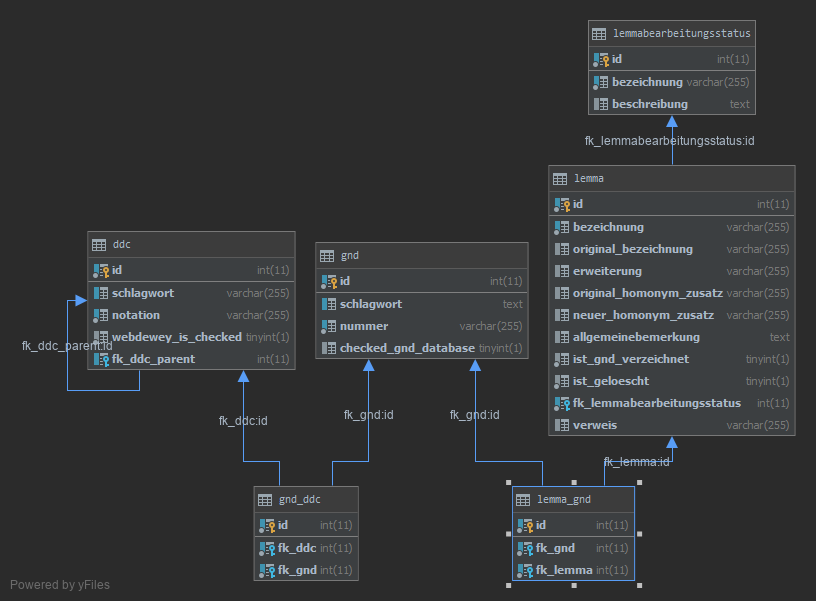
\includegraphics[width=0.8\linewidth]{images/structure_lemmaadministration.png}
	\caption{Tabellenaufbau der Lemma-Administration Übersicht.}
	\label{img:lAdminStructure}
\end{figure}

\begin{figure}
	\centering
	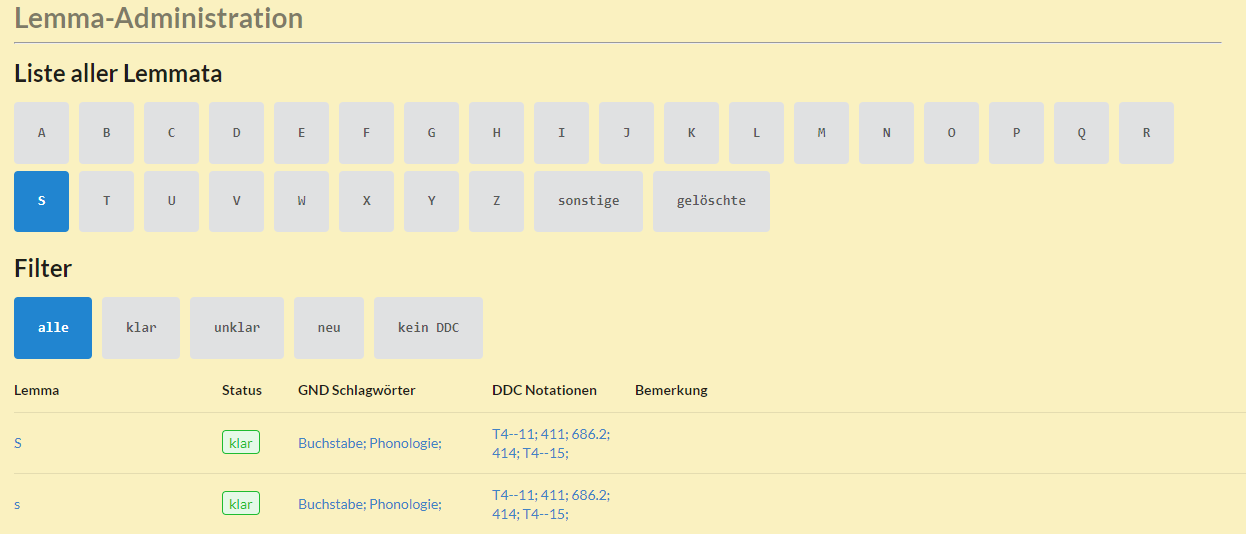
\includegraphics[width=1\linewidth]{images/lemmaadministration_sample.PNG}
	\caption{Frontend Ansicht der Lemma-Administration mit geladenen Buchstaben S (Ausschnitt).}
	\label{img:lAdminSample}
\end{figure}

\lstset{language=SQL}
\begin{lstlisting}[frame=single] 
    SELECT
    lemma.id
FROM lemma
WHERE
    lemma.bezeichnung LIKE 'S%'
    AND lemma.ist_geloescht = 0
ORDER BY
    lemma.bezeichnung ASC,
    lemma.id ASC;
\end{lstlisting}

Im zweiten Schritt werden dann die gerade geholten ID’s mit vielen JOIN’s für die Darstellung vorbereitet.

\lstset{language=SQL}
\begin{lstlisting}[frame=single] 
SELECT  lemma.id,                        
        lemma.bezeichnung,                
        lemma.original_bezeichnung,     
        lemma.erweiterung,               
        lemma.original_homonym_zusatz,  
        lemma.neuer_homonym_zusatz,      
        lemma.allgemeinebemerkung,       
        lemma.ist_gnd_verzeichnet,      
        lemma.ist_geloescht,             
        lemma.verweis,                  
        lemma.fk_lemmabearbeitungsstatus, 
        lemmaBStatus.id,               
        lemmaBStatus.bezeichnung,    
        lemmaBStatus.beschreibung,              
        lemma_gnd_map.id,                 
        gnd.id,               
        gnd.nummer,                   
        gnd.schlagwort,             
        gnd_ddc_map.id,              
        ddc.id,                      
        ddc.notation,               
        ddc.schlagwort,             
        ddc.webdewey_is_checked,        
        lemma.fk_lemmabearbeitungsstatus,
        lemma_gnd_map.fk_lemma,
        lemma_gnd_map.fk_gnd,          
        gnd_ddc_map.fk_gnd,         
        gnd_ddc_map.fk_ddc,                
        ddc.fk_ddc_parent            
FROM lemma lemma
      
INNER JOIN lemmabearbeitungsstatus lemmaBStatus
ON lemma.fk_lemmabearbeitungsstatus = lemmaBStatus.id

LEFT JOIN lemma_gnd lemma_gnd_map ON lemma.id = lemma_gnd_map.fk_lemma
LEFT JOIN gnd gnd ON lemma_gnd_map.fk_gnd = gnd.id
LEFT JOIN gnd_ddc gnd_ddc_map ON gnd.id = gnd_ddc_map.fk_gnd
LEFT JOIN ddc ddc ON gnd_ddc_map.fk_ddc = ddc.id
WHERE lemma.id IN ([Array of Lemma IDs])
ORDER BY lemma.bezeichnung ASC, lemma.id ASC;

\end{lstlisting}

Der zweite Query ist von dem Fehlermodul \ref{img:errorListSample}. Dieser Query verbindet die drei Tabellen \ref{img:errorListStructure} zu einer Darstellung. Es gibt für jeden Fehler einen Eintrag, dieser wird in tf\_fehler gespeichert. Da es für jeden Eintrag mehrere Fehler geben kann und diese Fehler für jeden Eintrag verfügbar sind, gibt es hier eine n zu m Beziehung. Um diese Abzubilden wurde die Tabelle tfl\_fehler\_rptmap eingefügt. Diese verbindet jeweils die ID’s mit den dazugehörigen Fehlercodes. 

\begin{figure}
	\centering
	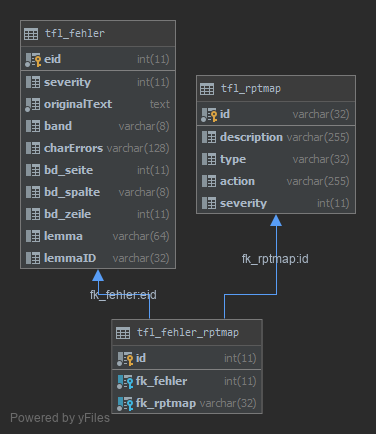
\includegraphics[width=0.5\linewidth]{images/structure_errormodule.png}
	\caption{Tabellenaufbau der Fehlerliste.}
	\label{img:errorListStructure}
\end{figure}

\begin{figure}
	\centering
	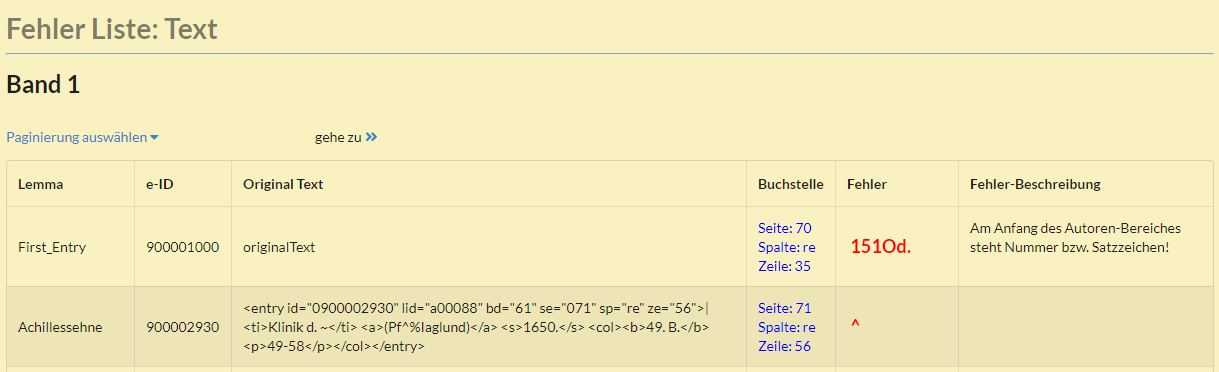
\includegraphics[width=1\linewidth]{images/errormodule_sample.png}
	\caption{Ansicht der Frontend Tabelle.}
	\label{img:errorListSample}
\end{figure}

\lstset{language=SQL}
\begin{lstlisting}[frame=single]  % Start your code-block

SELECT  fehler.eid,
        fehler.originalText,
        fehler.band,
        fehler.bd_seite,
        fehler.bd_spalte,
        fehler.bd_zeile,
        fehler.lemma,
        fehler.charErrors,
        fehlercodes.description
FROM tfl_fehler fehler

LEFT JOIN tfl_fehler_rptmap fehler_fehlercode_map 
ON fehler.eid = fehler_fehlercode_map.fk_fehler

LEFT JOIN tfl_rptmap fehlercodes 
ON fehlercodes.id = fehler_fehlercode_map.fk_rptmap

WHERE fehler.band = ('1')
AND fehler.severity > 3
ORDER BY fehler.eid;
\end{lstlisting}




\section{Solr}

\subsection{Installation}

Als Systemvoraussetzungen ist eine Java Version $> 8$ gegeben. Ich habe mich hierbei für OpenJDK 11 entschieden. 
Nach dem ersten Starten wurden 2 Warnungen gemeldet, dass die User-Limits für Solr zu gering sind \ref{lst:warningSolr}. Nachdem beide entsprechend erhöht wurden, verschwanden die Warnungen.

Um Solr im Entwicklermodus auszuführen, kann das entpackte Programm einfach mit \path{bin/solr start} gestartet werden. 

\begin{lstlisting}[language=bash, frame=single, label={lst:warningSolr}] 
    *** [WARN] *** Your open file limit is currently 1024.
    It should be set to 65000 to avoid operational disruption.

    *** [WARN] ***  Your Max Processes Limit is currently 63918.
    It should be set to 65000 to avoid operational disruption.
\end{lstlisting}

Die richtige Installation installiert Solr als Service und legt sich einen eignen Nutzer an. Ein entsprechendes Installations-Skript findet sich dafür im entpackten Solr-Ordner.

\subsection{Indexierung}

Um mit der Indexierung starten zu können, muss zuerst in sogenannter „Core“ erstellt werden. Dieser ist ein Index mit dazugehörigen Transaktionslog und Konfigurationsdateien. Nur mit diesen ist es möglich Dateien zu indexieren und auf ihnen zu suchen. Nach der Erstellung lässt sich der Core nun auch über die Oberfläche einsehen und zum Teil konfigurieren.

Damit Solr nun die Daten von der Datenbank liest, muss ein DataImportHandler (DIH) \ref{lst:dih} geschrieben werden. In diesen werden die Daten, welche Indexiert werden sollen mit MySQL-Queries eingelesen. Das System basiert dabei auf Entitys. Diese besizten jedeweils mehre Attribute, wie den Name, welcher auf der Oberfläche zur Indexierung angezeigt wird, den MySQL-Query mit dem die Daten gelesen werden und einen Delta-Query, welcher nur die neuen Einträge lädt. Der Delta-Query benötigt hierbei eine eigene Timestamp-Spalte in der Datenbank, welche angezeigt, wann die Spalte das letzte mal editiert worden ist. Da die Tabellen im Projekt eine solche Spalte nicht besitzen können die Delta-Querys nicht getestet werden. Innerhalb des Entity Elements gibt es entweder weitere Entitys, dazu gleich mehr, oder Field-Elemente. Diese besitzen ein Attribut, welches die Spalte der Tabelle ausweist und einen Namen, der das zugehörige Solr-Schema-Element ausweist. 
Entitys können unbegrenzt ineinander verschachtelt werden. Damit Änderungen an einer verschachtelten Entity nach oben richtig weitergegeben werden, gibt es ParentDeltaQuerys. Diese geben die betroffenen Werte an die übergeordnete Entity weiter. Dafür führt der ParentDeltaQuery einen Aufruf an die überliegende Entity-Tabelle aus in der er mithilfe der Femdschlüssel-Ids in den betroffen Zeilen herausfindet.

Der DataImportHandler muss, bevor er benutzt werden kann, jedoch noch mit dem Core verbunden werden, dafür wird er, zusammen mit einem JDBC-Treiber in die solrconfig.xml eingetragen. Bei den JDBC-Treiber habe ich mich bei diesem Beispiel für den Treiber von MariaDB entschieden. Damit es nicht deswegen zu Laufzeit-Unterschieden bei der Indexierung kommen kann, werde ich diesen Treiber bei allen Systeme mit JDBC-DataImportHandlern verwenden.

\begin{lstlisting}[language=xml, frame=single, label={lst:dih}, 
    morekeywords={entity,query,deltaQuery,parentDeltaQuery,field,column, name}] 
    <entity name="lemma" 
      query="select * from lemma" 
      deltaQuery="select eid from lemma 
        where last_modified > '${dataimporter.last_index_time}'"> 
		<field column="bezeichnung" name="bezeichnung" />
    [...]
    <entity name="lemma_gnd" 
      query="select * from lemma_gnd where fk_lemma='${lemma.id}'"
      deltaQuery="select * from lemma_gnd 
        where last_modified > '${dataimporter.last_index_time}'"
      parentDeltaQuery="select * from lemma 
        where id=${lemma_gnd.fk_lemma}">
			
        <entity name="gnd" 
          query="select * from gnd where id = '${lemma_gnd.fk_gnd}'"
          deltaQuery="select * from gnd 
            where last_modified > '${dataimporter.last_index_time}'"
          parentDeltaQuery="select * from lemma_gnd where fk_gnd=${gnd.id}">
          <field column="nummer" name="gnd_nummer" />
          <field column="schlagwort" name="gnd_schlagword" />
          [...]
        </entity>
      </entity>  
    </entity>
\end{lstlisting}

Wie schon eben angesprochen, muss das Solr-Schema für die entsprechende Elemente auch angepasst werden. Dieses Schema dient dazu die Dateitypen für eine möglichst gute Indexierung auszuweisen. Dafür wird zuerst der Dateityp für die Tabellen-Spalte angegeben. Dabei werden bei den Grundtypen, zum Beispiel unter anderem String und $text_de$ gelistet. Ohne genauer darüber nachzudenken, habe ich angenommen, dass beide gleichwertig sind und nur für spätere Abfragen auf Sprachen eine Relevanz besitzen. Als ich allerdings eine Abfrage stellte, die alle Lemmata mit den Buchstaben S finden sollte, bekam ich mehr Ergebnisse als erwartet. Dies liegt daran, dass $text_de$, das Feld aus Volltext ausweißt. Deswegen wird jedes Wort als einzelne Entity gewertet und so kamen Lemma, in welchen irgendein Wort mit S begann in meine Auflistung. Auch muss darauf geachtet werden, ob man String oder Strings als Typen angibt, letzteres weist das Feld als multiValued aus, bildet also eine 1 zu N Beziehung ab. So kann man zusammen mit der Verschachtelung N zu M Beziehungen abbilden. Genaueres zu diesem Thema allerdings in Kapitel !!Kapitel anfügen!!.
Um diese Einträge auszuweisen gibt es mehrere Möglichkeiten. In diesem Fall habe ich die Einträge über die Administrations-Oberfläche angelegt. Es ist allerdings auch möglich eine eigenen Shema-Datei zu erstellen. Diese Methode soll allerdings nicht mehr verwendet werden, da es die Möglichkeit gibt, diese Einträge per API einlesen zu lassen. Dabei wird direkt überprüft, ob die Einträge formal stimmen. So können keine fehlerhaften Schemata gebaut werden. Die Einträge, welcher über die API oder die Administrations-Oberfläche gestellt werden, werden in einer Datei names $managed_schema$ im XML-Format angelegt \ref{lst:managedSchema}.


\begin{lstlisting}[language=xml, frame=single, label={lst:managedSchema}, 
    morekeywords={type,uninvertible,indexed,stored,field,multiValued, name}] 

    [...]
    <field name="ddc_webdewey_is_checked" type="boolean" 
        uninvertible="false" indexed="true" stored="true"/>
    <field name="description" type="text_de" uninvertible="false" 
        multiValued="true" indexed="true" stored="true"/>
    <field name="erweiterung" type="text_de" 
        uninvertible="false" indexed="true" stored="true"/>
    [...]

\end{lstlisting}

Die Indexierung lief eine Minute und 34 Sekunden für run 14 Tausend Einträge \ref{img:solrIndexTime}. Dabei wurde der gegebene Arbeitsspeicher nicht komplett ausgenutzt, was darauf schließen lässt, dass die Datenbank der limitierende Faktor war. Die hohe Anzahl der Abfragen ist darauf zurückzuführen, dass Solr keine Joins verwendet, sondern bei jeder verschachtelten Entity die gesammte Tabellen nach passenden Einträgen durchsucht.

\begin{figure}
	\centering
	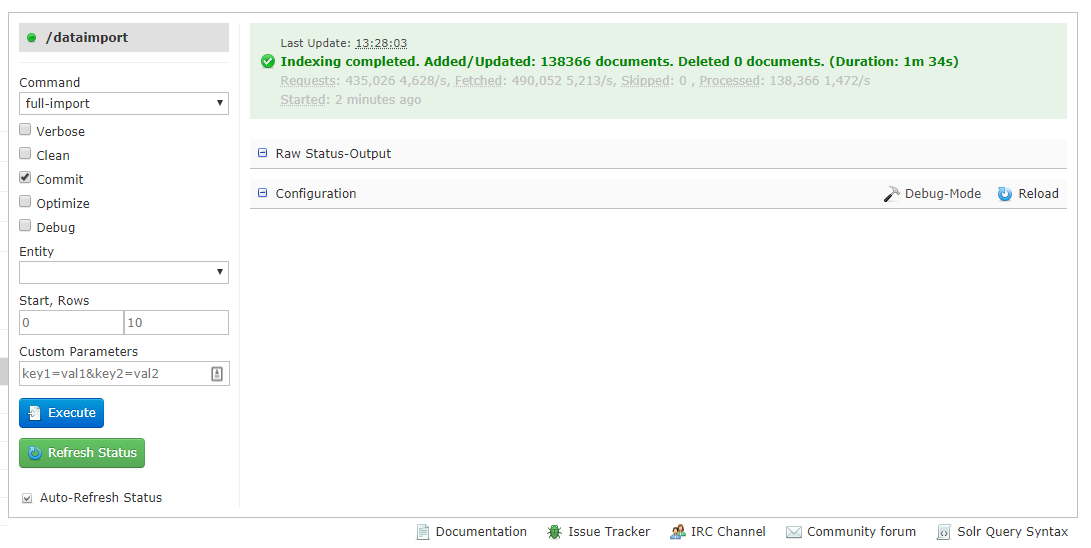
\includegraphics[width=1\linewidth]{images/solr_indexing_time.png}
	\caption{Indexierungsoberfläche mit Laufzeit.}
	\label{img:solrIndexTime}
\end{figure}

\subsection{Oberfläche}

Der Startseite des Solr-Systems bietet direkten Einblick in auf die Auslastung des Systems. Der Fehler-Log ist auch sehr einfach mit einem Klick zu erreichen. Um Statistiken zu dem aktuellen Core zu bekommen, kann dieser aus einen Drop-Down-Menu ausgewählt werden. Positiv anzumerken ist, dass es möglich ist das Schema direkt in der Weboberfläche zu modifizieren. Leider ist es nicht möglich, den DataImportHandler direkt zu verändern, ohne weitere Einstellungen im System vorzunehmen. Es gibt eine Möglichkeit Querys direkt über den Web-Client zu senden, was zum Testen und debuggen sehr nützlich ist. Auch bei der Indexierung kann ein Debug-Modus dazu geschaltet werden \ref{img:solrIndexTime}. Zudem gibt es die Möglichkeit die Konfigurationsdateien des Cores auf der Weboberfläche einzusehen, jedoch ist eine Editierung nicht möglich.
Es gibt keine Möglichkeit Updates direkt über die Weboberfläche einzuspielen, zudem ist die Seite auch nicht responsive geschrieben. 

\begin{figure}
	\centering
	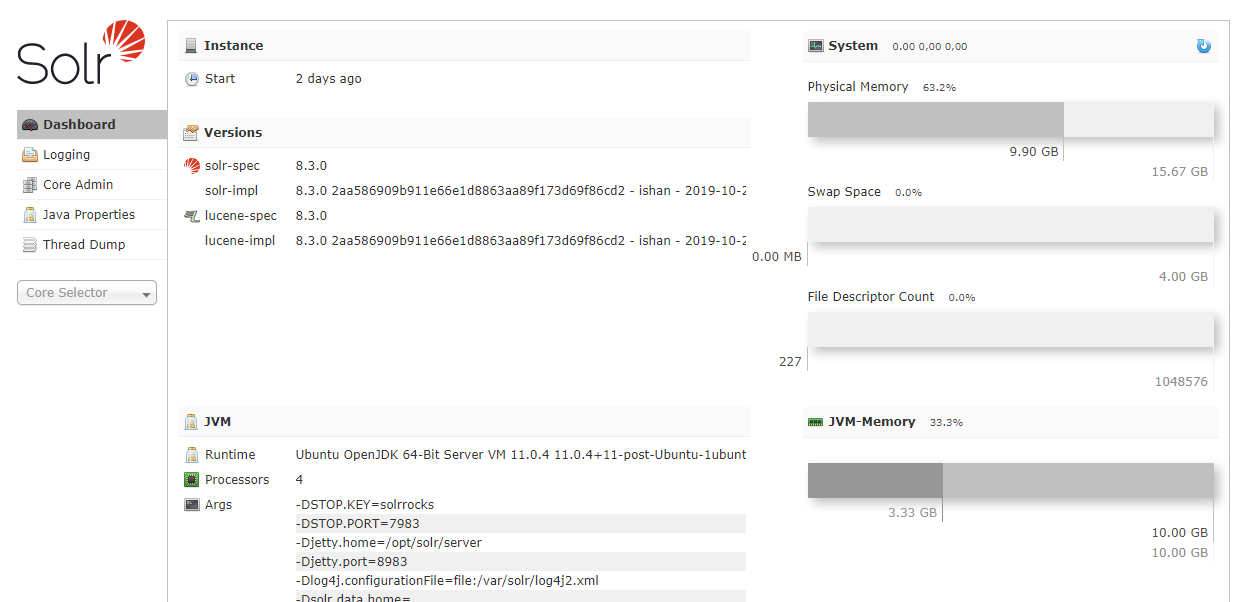
\includegraphics[width=1\linewidth]{images/solr_interface.png}
	\caption{Startseite der Weboberfläche von Solr.}
	\label{img:solrInterface}
\end{figure}


\subsection{Dokumentation}

Die Dokumentation war bei diesen kurzen Test meine Hauptquelle, die Installation ist dort sehr genau beschrieben. Positiv aufgefallen ist dabei vorallem die genaue Beschreibung der Systemanforderungen. Generell gibt es für alle Themen eine kleine Übersichtsseite, welche die grundlegenden Funktionen erklärt, ohne sich dabei in Details zu verlieren. 
Die Seite für den DataImportHandler hat anhand eines Beispiels gut die Struktur des Handlers abgebildet. Allerdings wäre ein Verweis, dass für die DataImportHandler-Attribute noch extra ein Solr-Schema-Attribut benötigt wird, schön gewesen. Dies habe ich erst durch einen Blog \cite{IqubalMustafaKaki.2016} herausgefunden und richtig verstanden. 
Die Dokumentation ist zum Reinlesen in die Grundlagen des Systems vollkommen ausreichend und bietet mit den Übersichtsseiten für die einzelnen Themen einen guten Startpunkt.

\subsection{Absetzen einer Anfrage und Integration in PHP}

Um nicht direkt mit der JSON-API arbeiten zu müssen, gibt es diverse Bibliotheken, die einige Arbeit abnehmen. Eine der größten ist hierbei Solarium, welches sich über Composer installieren lässt. Dies passt sehr gut zum Dietrich-Online Projekt, da auch dieses auf Composer aufbaut. Die Query ist herbei sehr einfach, da die Daten beim Import schon für diesen Query optimiert wurden.

\begin{lstlisting}[language=php, frame=single, label={lst:managedSchema}, 
  morekeywords={type,uninvertible,indexed,stored,field,multiValued, name}] 

  [...] # Imports and variable declarations

  $config = array(
      'endpoint' => array(
          'localhost' => array(
              'host' => '136.199.34.55',
              'port' => 8983,
              'core' => 'dietrich'
  )));
  $queryText = 'original_bezeichnung:S*';
  $solr = new Client($config);
  $query = $solr->createSelect();
  $query->setQuery($queryText);
  $query->setRows(2147483647); 
  [...] # Loop with Timer
  $resultSet = $solr->select($query);
  $count = $resultSet->count();
  [...] # Output Runtime
\end{lstlisting}

Interessant bei der Verbindung ist, dass die Anzahl der Zeilen die von Solr geladen werden, standardmäßig auf 10 limitiert sind. Erst mit setRows kann die Anzahl erhöht werden. Ich habe hierfür den maximalen Integer-Wert gewählt, um immer alle Ergebnisse zu bekommen. Um bei diesen Test nun einen guten Median-Wert zu erhalten, habe ich die Abfrage 100 mal laufen lassen. Dabei lieft die Abfrage durchschnittlich 1.01 Sekunden um die 15838 Ergebnisse herauszusuchen. Eine Vergleichtabelle, wie sich Solr dabei mit den anderen Suchmaschinen schlägt, finden Sie hier. !!VERGLEICH ANFÜGEN!!


\section{Datafari}

Die zweite Suchmaschine, welche verglichen wird ist Datafari von France Labs.

\subsection{Installation}

Für Datafari musste die folgende Software nachinstalliert werden: Java 8 und JQ, ein JSON-Prozessor. Damit die Installation korrekt funktioniert, muss die JAVA\_HOME-Variable erstellt werden. Insofern Datafari nicht unter Root laufen soll, muss noch ein besonderer Nutzer mit Root Rechten angelegt werden. Dieser muss, wie schon bei Solr, höhere User-Limits erhalten. Datafari installiert sich selbständig durch eine DEB-Datei. Während der Installation erscheint ein kurzer Setup-Dialog, mit welchem durch die Konfiguration geführt wird. Das Starten des Server geschieht daraufhin durch ein Script im Installationsordner.

\subsection{Indexierung}

Damit eine Indexierung durchgeführt werden kann, muss bei Datafari ein sogenanntes Repository angelegt werden. In diesem wird die Datenbankverbindung eingetragen. Dabei ist es wichtig, dass vorher der Treiber korrekt installiert wird. Dabei kam es zu Problemen.
Das auf Apache ManifoldCF basierende System akzeptiert nur MySQL-JDBC Treiber. Da der MariaDB-Treiber einen anderen Klassennamen in Java verwendet, funktioniert dieser nicht. \begin{quote} This connection type cannot be configured to work with other databases than the ones listed above without software changes.~\cite[S.~61]{ApacheSoftwareFoundation.}\end{quote} Deswegen wurde für diesen Test den MySQL-Treiber von Oracle verwendet.
Nachdem der Treiber korrekt installiert wurde und das Repository erstellt war, kann nun einen Job zur Indexierung der Einträge gestartet werden. In diesem werden die Abfragen und der Zeitplan konfiguriert.
Im ersten Schritt wird das Repository und das Ziel ausgewählt. In dem Tab Querys lassen sich dann diverse Abfragen bauen. Der erste ist ein Seeding-Query, welcher eine Art Delta-Query für dieses System ist. Als Nächstes wird der Data-Query benötigt, welcher die Daten aus der Datenbank lädt. Dabei werden mehrere Variablen definiert, damit der Query korrekt von ManifoldCF erkannt wird. 

Zuerst einmal das Feld: IDCOLUMN, welches die ID enthält, dann URLCOLUMN, welches einen Hyperlink für diesen Eintrag enthält. Da hier keine solche Spalte gegeben ist, wird einfach nochmal die ID mitgegeben, was so in einen Screenshot aus der Dokumentation zu sehen ist. Zuletzt noch die DATACOLUMN, welche alle Daten konkateniert enthält. Um das System zu testen habe ich allerdings erstmal nur eine Zeile in die DATACOLUMN geschrieben \ref{img:datafariQuery}. Die Konkatenation ist vorgegebene die Methode aus der ManifoldCF-Dokumentation. \cite[S.~97]{ApacheSoftwareFoundation.} Dies ist für unseren Zweck keine saubere Datenstruktur.
Sind alle Querys eingetragen, kann die Indexierung beginnen. Dafür wird der Job in der Oberfläche manuell gestartet, insofern kein Zeitplan konfiguriert ist.

In diesem Test kam es dabei allerdings zu Problemen. Die Indexierung erfolgte nicht korrekt und blieb immer am Ende hängen. Der Log zeigte ein „Ready for processing“ an, machte dort allerdings nicht weiter. Einen Eintrag in der Dokumentation oder generell im Internet konnte nichts gefunden werden. Auch eine Reduktion der Einträge auf nur 125 hat das Problem leider nicht lösen können. Deswegen wurde der Test an dieser Stelle abgebrochen. 

\begin{figure}
	\centering
	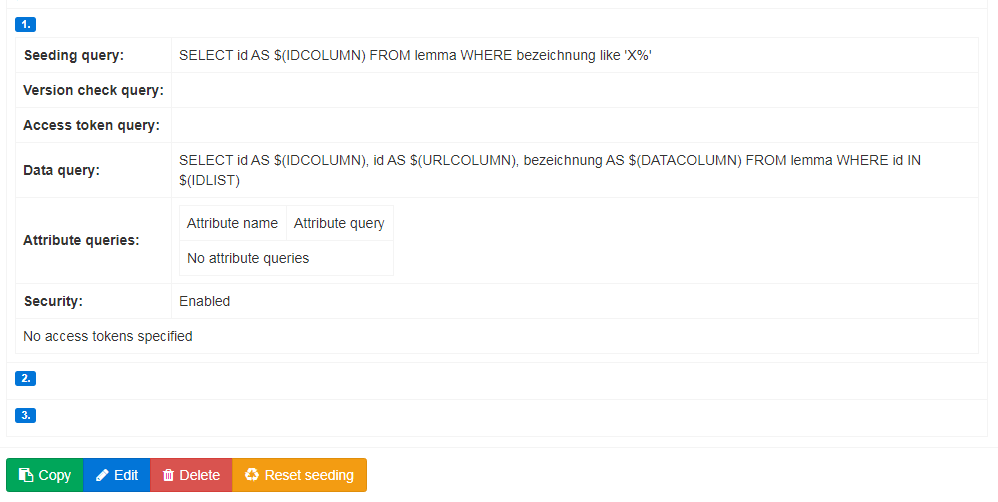
\includegraphics[width=1\linewidth]{images/datafari_query.png}
	\caption{Übersichtsseite des Querys in Datafari.}
	\label{img:datafariQuery}
\end{figure}

\subsection{Oberfläche}

Die Oberfläche von Datafari ist dreigeteilt. Zum einen gibt eine Such-Oberfläche, welche sich ohne Anmeldung erreichen lässt. 

Als Zweites findet sich eine Administrationsoberfläche, welche erst eingesehen werden kann, sobald man eingeloggt ist. Dort findet finden sich diverse Einstellungen für die Suchmaschine, wie Synonyme oder die Facetten-Konfiguration. Auch sind dort die Logs einzusehen, welche durch über Kibana \ref{elasticsearch} angezeigt werden. 

Die dritte Oberfläche ist die Einstellungsseite für die Datacrawler. Dies ist eine modifizierte Oberfläche von Apache ManifoldCF. Generell sind die Menüs sehr übersichtlich, auch wenn die Einbindung von anderen Anwendungen keine Ideale Lösung darstellt. Es lassen sich keine Updates direkt über die Oberfläche einspielen.
Die Such-Seite und die Seite für die Erstellung der Datacrawler sind Responsive, während die Administrationsoberfläche bei kleineren Bildschirmgrößen das Menü versteckt und die Seite somit unnutzbar macht.

\begin{figure}
	\centering
	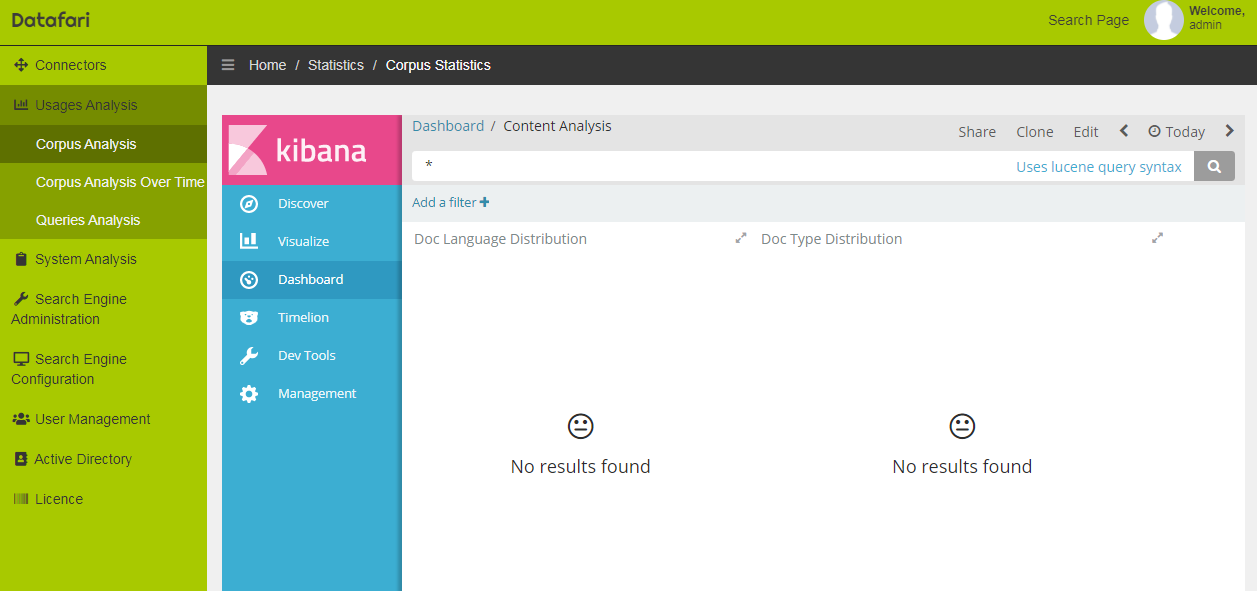
\includegraphics[width=1\linewidth]{images/datafari_kibana.png}
	\caption{Kibana Integration in Datafari.}
	\label{img:datafariKibana}
\end{figure}

\subsection{Dokumentation}

Die Dokumentation geht sehr genau auf die Installation des Systems ein. Dabei werden alle Konfigurationsaspekte beleuchtet. Es wird zum Beispiel beschrieben, wie die User Limits erhöht werden können, oder wie die JAVA\_HOME-Variable korrekt gesetzt wird. Allerdings ist an manchen Stellen zu merken, dass die Dokumentation nicht von nativ Englischsprechenden geschrieben wurde, da die Grammatik nicht immer korrekt ist. Allerdings hat dies nicht zu Problemen oder Verwechslungen geführt.

Bei der Dokumentation zum Einrichten des JDBC-Treibers finden sich einige Probleme \ref{img:datafariJDBC}. Zum einen sind beide Pfade, die in dem Text angegeben sind, falsch. Einer davon wird sogar richtig in dem Screenshot direkt darunter angezeigt. Und zum anderen ist der zweite Screenshot so niedrig aufgelöst, dass sich kaum etwas erkennen lässt. Dies passiert auch, wenn das Bild in einen neuen Tab geladen wird. Generell ist die Dokumentation für den Umgang mit Datenbanken nicht sehr ausführlich. Die Erklärungen, wofür die Variablen bei der Erstellung eines Jobs stehen, mussten in der Dokumentation von ManifoldCF nachgelesen werden.

Die Dokumentation ist im aktuellen Stand nicht sauber strukturiert. Sie gibt das Gefühl, dass es sich eher um eine Sammlung verschiedener Artikel, welche Intern genutzt wurden, handelt.

\begin{figure}
	\centering
	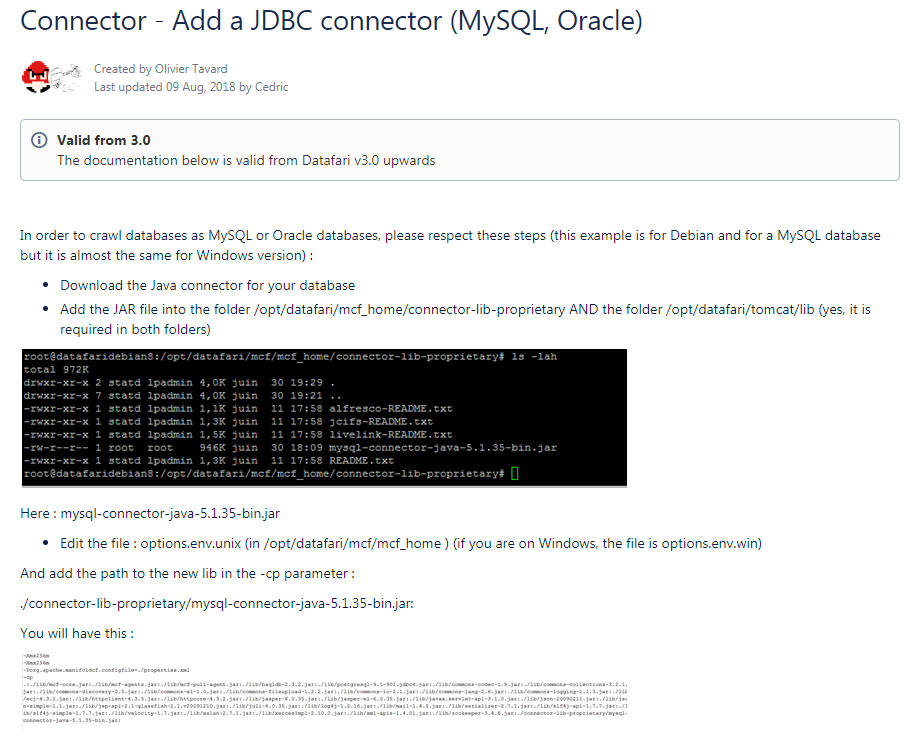
\includegraphics[width=1\linewidth]{images/datafari_doku_wrong_path.png}
	\caption{Dokumentationsseite für den JDBC Treibers von Datafari.}
	\label{img:datafariJDBC}
\end{figure}


\subsection{Absetzen einer Anfrage und Integration in PHP}

Durch das fehlgeschlagene Einlesen der Daten konnte dieser Test nicht durchgeführt werden.


\section{ElasticSearch}

\subsection{Installation}

Die Installation ist bei ElasticSearch dreigeteilt. Um die Suchmaschine in dem Umfang nutzen zu können, wie es hier benötigt wird, muss der komplette ELK-Stack installiert werden. ElasticSearch ist hierbei das Kernstück und dient als Datenbank. Kibana ist eine grafische Benutzeroberfläche und Logstash bildet die Brücke zwischen der MySQL-Datenbank und ElasticSearch. Während ElasticSearch Java mitgeliefert hat, muss für Logstash Java Version 8 oder 11 nachinstalliert werden. Um die drei Dienste für den Development Modus zu installieren, müssen nur die Archive entpackt und die entsprechenden Anwendungen gestartet werden. Ohne die Konfigurationsdateien zu ändern, haben die Anwendungen direkt miteinander kommunizieren können. Allerdings gab es bei Logstash ein paar Warnungen beim Start, welche mit JRuby zusammenhingen und den Entwicklern schon bekannt sind. Daher können diese hier ignoriert werden.

Für eine richtige Installation gibt es mehrere Wege, entweder man fügt deren Repository ein, verwendet das bereitgestellte Debian-Paket oder installiert per Docker. Für diesen Test habe ich mich für das Debian-Paket entschieden. Die Installation verlief dabei ohne weitere Probleme.

\subsection{Indexierung}

Um nun Daten zu indexieren, muss in einer Conf-Datei in Logstash definiert werden, wie und welche Daten gelesen und weitergegeben werden sollten \ref{lst:lsConf}. Dabei kann Logstash direkt MySQL-Querys gegen die Datenbank stellen. Die Datei ist in zwei Blöcke unterteilt. Zum einen ein Input-Block, welcher erklärt, welche Daten eingelesen werden sollen und einen Output Block, welcher das Ziel für die Daten angibt. Für den Input Block verwende ich hier den MariaDB-Treiber.

Bei diesem Schritt kam es bei dem System allerdings zu Problemen. Der Treiber konnte über den in der Dokumentation angegeben Weg nicht geladen werden.  Damit der Treiber korrekt erkannt werden konnte, musste er zusammen mit den Core-Bibliotheken von Logstash geladen werden. Deswegen ist die Zeile mit dem Pfad zur Bibliothek auch leer. 

Nachdem die Datenbank Konfiguration und Query angegeben wurden, kann zudem noch ein Zeitplan definiert werden. Außerdem ist es auch möglich, eine Art Delta-Query zu definieren. Hierfür wird eine Tracking-Spalte festgelegt, welche dann in der Query auf einen Zeitstempel überprüft wird.

Im zweiten Teil der Datei wird das Ziel definiert. Die erste Zeile dient dazu nur dem Debugging, da es alle ausgegeben Linien des Skripts auch auf die Shell ausgibt. In dem ElasticSearch-Segment wird zum einen eine ID definiert, welche verhindert, dass Einträge doppelt in die Datenbank gespielt werden. Deswegen wird hier die ID der Lemmata genommen, da diese auch in der Datenbank nicht wiederholt werden darf. Zum anderen wird noch ein Index angegeben, welcher für die erhaltenen Daten angelegt wird. 

Als die Indexierung nun gestartet wurde, kam es allerdings zu einem Fehler, dass die MySQL-Query nicht gültig sei. Um zu ermitteln, wie viele Daten indiziert werden müssen, wird die Query mit einer Count-Abfrage umhüllt. Dabei verwendete Logstash Double anstelle von Single-Quotes, was bei MariaDB zu einem Fehler führte. Dies konnte behoben werden, indem eine Einstellung in der Datenbank vorgenommen wurde, um auch Double-Quotes zu erlauben. 
Danach verlief die Indexierung ohne weitere Probleme.

\begin{lstlisting}[language=xml, frame=single, label={lst:lsConf}] 
  input {
    jdbc {
      jdbc_validate_connection => true
      jdbc_driver_library => ""
      jdbc_driver_class => "Java::org.mariadb.jdbc.Driver"
      jdbc_connection_string =>
          "jdbc:mariadb://localhost:3306/dietrichonline"
      jdbc_user => "USER"
      jdbc_password => "PW"
      tracking_column => "timestamp"
      use_column_value=>true
      statement => "MYSQL-Query WHERE timestamp > :sql_last_value"
      schedule => "0 */6 * * *"
    }
  }
  
  output {
    stdout { codec => json_lines }
    elasticsearch {
      document_id => "%{id}"
      index => "lemma"
      hosts => "localhost:9200"
    }
  }
\end{lstlisting}

Nun ist die Frage jedoch, wie weiß ElasticSearch, was für ein Datentyp das Feld besitzt. Dafür verwendet ElasticSearch ein sogenanntes Dynamic-Mapping, indem es versucht den am besten passenden Datentyp für das Feld zu ermitteln.

Um eigene Feld-Typen zu setzen, muss der Index von Hand erstellt werden. Um ein Feld zu definieren, muss ein Mapping manuell erstellt werden \ref{lst:mapping}. Dieses enthält zumindest den Feld-Namen und den Typen. Zudem können noch andere Optionen angegeben werden, um die Indexierung nach dem eigenen Ermessen anzupassen. Es kann zum Beispiel deklariert werden, dass ein Feld zwar existiert, allerdings nicht Suchbar ist. Dies ist für IDs interessant, die zur Verwaltung der Indices dienen, allerdings nicht nach außen hin herausgegeben werden sollen.

\begin{lstlisting}[language=xml, frame=single, label={lst:mapping}] 
PUT lemma
{
  "mappings": {
    "properties": {
      "original_bezeichnung": {
        "type":  "keyword"
}}}}
\end{lstlisting}

Will man allerdings nicht alle Felder von Hand erstellen, ist es zudem möglich eine Vorlage für ein dynamisches Feld zu generieren \ref{lst:mappingTemplate}. So kann für ein Feld eine bestimmte Regel gesetzt werden, ohne alle Felder manuell anlegen zu müssen. Als Beispiel habe ich hier definiert, dass das Feld original\_bezeichnung immer nur als Keyword gespeichert wird.

\begin{lstlisting}[language=xml, frame=single, label={lst:mappingTemplate}] 
PUT lemma
{
  "mappings": {
    "dynamic_templates": [
      {
        "obez_as_keyword": {
          "match":   "original_bezeichnung",
          "mapping": {
            "type": "keyword"
  }}}]}}
\end{lstlisting}

Für den Test war eine Erstellung eines Mappings oder eines dynamischen Templates allerdings nicht notwendig, da ElasticSearch bei der automatischen Indexierung jedes String-Feld als Keyword, sowie Volltext abspeichert, insofern die Länge unter 256 Zeichen ist.

\subsection{Oberfläche}

Die Oberfläche von Kibana bietet eine zu Beginn überwältigende Erfahrung \ref{img:elasticInterface}. Um dies für spätere Anwender zu verhindern, bietet Kibana die Möglichkeit Sichten für unterschiedliche Nutzer zu erstellen. Zudem kann die Oberfläche hinter ein Login-System geschaltet werden.

Auf der Oberfläche gibt es viele Menüpunkte, welche es ermöglichen die Daten auf diverse Arten darzustellen, darunter in Grafen-Form oder auf einer Landkarte. Unter dem Punkt Management finden sich die Einstellungen für das ElasticSearch System. Hier kann man nicht nur Snapshots erstellen, sondern auch das System mit Updates versorgen. Zudem können hier die Indices verwaltet werden \ref{img:elasticIndexSettings}. Eine Erstellung der Indices ist allerdings nur per API möglich. Allerdings ist es möglich einige Einstellungen an den Indices vorzunehmen und diese auch zu löschen. Zudem gibt es die Möglichkeit Indices eine Lebensdauer zuzuweisen, was in Zeiten der Datenschutzgrundverordnung sicherlich eine nützliche Funktion darstellen wird. 

Die Oberfläche ist vollkommen responsive. Neben diesem Menü gibt es ebenfalls eine Entwicklerkonsole, in der es möglich ist Anfragen an das ElasticSearch-System zu schicken, ohne mit Curl oder ähnlichen zu arbeiten, was das Debugging vereinfacht.

\begin{figure}
	\centering
	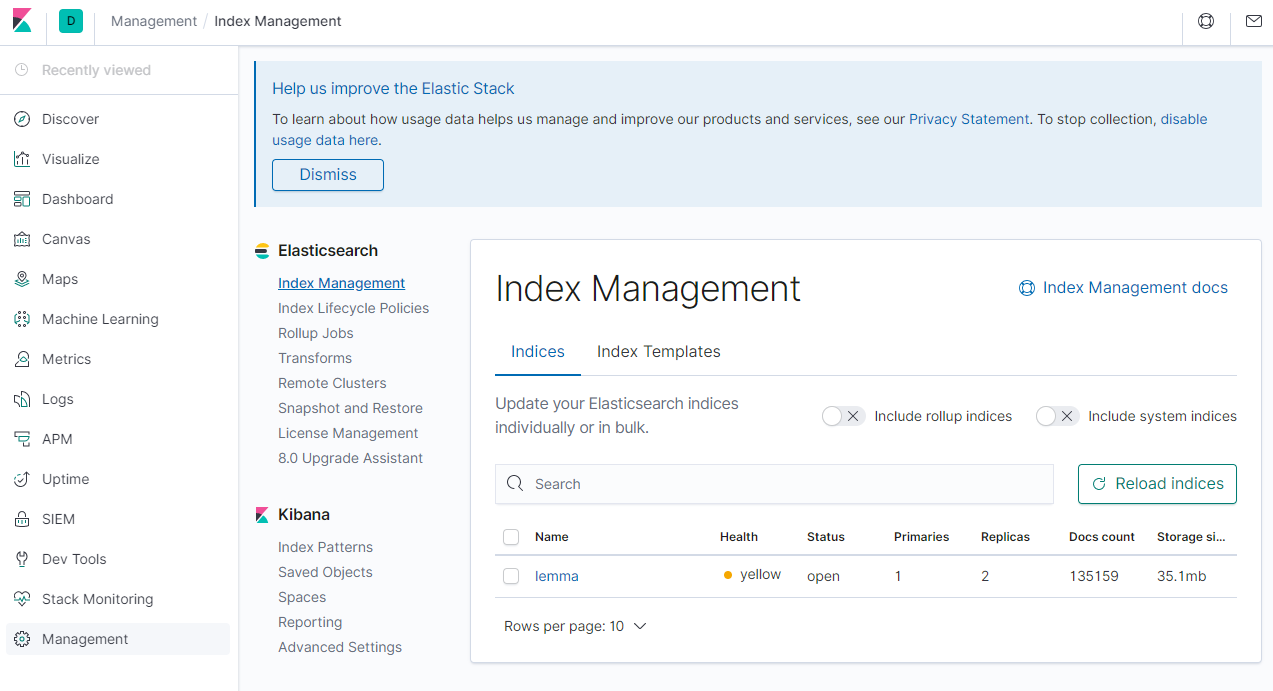
\includegraphics[width=1\linewidth]{images/elastic_ui.png}
	\caption{Index Management Seite von ElasticSearch}
	\label{img:elasticInterface}
\end{figure}


\subsection{Dokumentation}

Die Dokumentation von ElasticSearch ist sehr ausführlich und gut zu lesen. Um einen einfacheren Einstieg in das System zu bieten, beginnt die Dokumentation bei jedem Thema mit einem kleinen Beispiel, um das Konzept zu verdeutlichen. Diese Struktur zieht sich durch die gesamte Dokumentation, jedes Thema ist mit vielen Codeschnipseln bebildert, was eine einfachere Einarbeitung in das System ermöglicht. 
Gut gelöst dabei ist, dass es möglich ist mit einem Klick den Befehl direkt in die Konsole von Kibana zu importieren. Während meines Testes ist mir nur ein Fehler in der Dokumentation aufgefallen, und zwar wurde bei der Informationsseite zum PHP-Klienten eine falsche PHP-Version vermerkt.


\subsection{Absetzen einer Anfrage und Integration in PHP}

ElasticSearch bietet für PHP einen eigenen Klienten an. Es ist möglich, diesen unter anderem auch mit Composer zu installieren. Um die indexierten Dateien abzufragen, muss ein ClientBuilder gebaut werden, welcher einen oder mehrere Hosts mitgegeben bekommt. Der Server sendet, insofern nicht anders konfiguriert, 10 Resultate zurück. Um diese Limitierung aufzuheben, muss hierbei an 2 Stellen etwas verändert werden. In PHP muss dem Klienten bei der Anfrage ein Parameter mitgegeben werden, welcher die Menge der Ergebnisse bestimmt. Dies funktioniert allerdings nur bis zu 10.000 Ergebnissen. Sollten mehr Ergebnisse erwünscht sein, muss auch noch etwas am Index geändert werden. Dies kann entweder über eine HTTP Anfrage oder über die Oberfläche geändert werden. Für den Test wurde dieses Limit nun erhöht \ref{img:elasticIndexSettings}. 


\begin{lstlisting}[language=php, frame=single, label={lst:phpElastic}, 
  morekeywords={type,uninvertible,indexed,stored,field,multiValued, name}] 
  <?php
  [...] # Imports and variable declarations

  $clientBuilder = ClientBuilder::create()->setHosts(['136.199.34.55']);
  $client        = $clientBuilder->build();

  $params = [
      'index' => 'lemma',
      'body' => [
          'size' => 1000000,
          'query' => [
              "wildcard" => ["bezeichnung.keyword" => "S*"],
  ]]];
  
  $results = $client->search($params);
  [...] # Loop with Timer  
  $results = $client->search($params);

  $count=0;
    foreach ($results['hits']['hits'] as $hit){
      $count++;
    }
  [...] # Output Runtime
  
\end{lstlisting}

Zum Code ist noch zu sagen, dass im Ergebnis keine Summe der Ergebnisse liegt, sondern dafür ein eigener Query vonnöten ist. Deswegen werden hier die Ergebnisse in einer Schleife gezählt.

Auch hier wurde nun der Query 100-Mal ausgeführt, um einen Median Wert zu ermitteln. Dieser lag bei ElasticSearch bei 0.58 Sekunden pro Query und erbrachte 15653 Ergebnisse bei jeden Durchlauf.

\begin{figure}
	\centering
	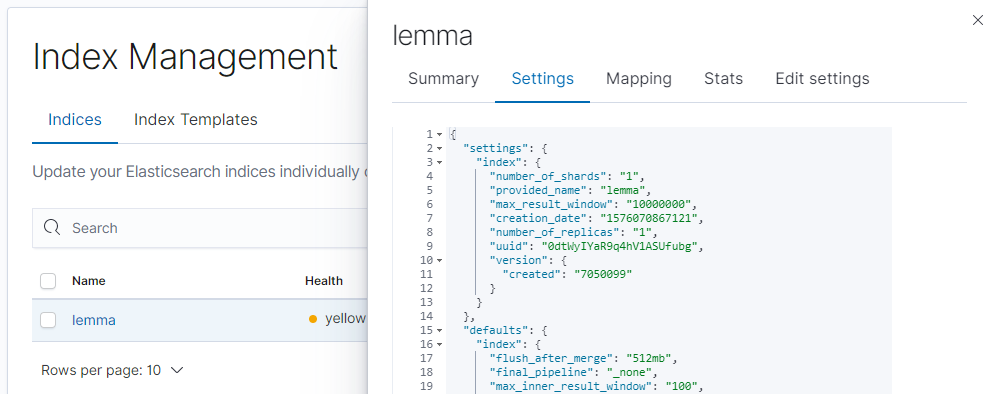
\includegraphics[width=1\linewidth]{images/elastic_index_settings.png}
	\caption{Einstellungen vom Lemma-Index bei ElasticSearch}
	\label{img:elasticIndexSettings}
\end{figure}




\section{Xapian}

\subsection{Installation}

Der empfohlene Installationsweg für Xapian führt über die Paketquelle (PPA) der Entwickler. Nachdem dieses eingefügt wurde, kann Xapian entweder in einer C++ oder Python Variante installiert werden. 

Um die Suchmaschine auch über PHP anzusprechen ist es notwendig, den PHP-Connector aus Lizenzgründen selbst zu bauen. Dabei muss vorher ein Eintrag, der ausweist, dass aus dieser Quelle auch Source-Code geladen werden kann, in den Paketquellen hinzugefügt werden. Danach kann der Klient mithilfe von Make gebaut werden.

Allerdings ist der Server bisher nur lokal ansprechbar. Um dies zu ändern, muss ein TCP-Server für Xapian gestartet werden. Um diesen zu nutzen ist es vonnöten, ein weiteres Paket aus der Paketquelle zu installieren. Damit der Server gestartet werden kann, muss zuerst ein Index, der bei Xapian Database genannt wird, gebaut werden. Dazu mehr in dem Teil \ref{xap:index}. Danach kann der Server auf einen beliebigen Port gestartet werden.

\subsection{Indexierung}
\label{xap:index}

Durch die fehlende Dokumentation zur Indexierung von MySQL-Datenbanken, wurde erstmal ein Beispiel zum Import einer CSV-Datei durchgearbeitet. Darin war dann zu sehen, dass der komplette Datenimport manuell geschrieben werden musste. Auf dieser Basis wurde daraufhin ein eigener Importer für MySQL geschrieben \ref{lst:XapPhp}:

\begin{lstlisting}[language=php, frame=single, label={lst:XapPhp}, morekeywords={type,uninvertible,indexed,stored,field,multiValued, name}, caption=Skript zur Indexierung der Daten in Xapian,captionpos=b] 
<?php
require_once("xapian.php");

//Open MYSQL-Connection and Run Query. Save the Output in $result

// Create or open the database we're going to be writing to.
$db = new XapianWritableDatabase($xapianDb, Xapian::DB_CREATE_OR_OPEN);
// Set up a TermGenerator that we'll use in indexing.
$termgenerator = new XapianTermGenerator();
$termgenerator->set_stemmer(new XapianStem('de')); //Setup Stemmer

while ($row = $result->fetch_assoc()) { //Loop through MySQL-Rows

	$identifier = $row['id'];
	unset($row['id']);
	// Create new Row for the starting Letter
	$searchIndexLetter = $row['original_bezeichnung'][0];

	$doc = new XapianDocument(); // Create new Document
	$termgenerator->set_document($doc); //Put it into the Term-Generator

	// Index the field with a suitable prefix.
	$termgenerator->index_text($searchIndexLetter, 1, 'K'); 
	// Make it available for Search
	$termgenerator->index_text($searchIndexLetter); 

	foreach ($row as $index) {
		if ($index = '') { //Xapian cant Index Empty Fields
			$index = 'EMPTY';
		}
		$termgenerator->increase_termpos(); // Make Space between Entries
		$termgenerator->index_text($index); // Add Every Field
	}
	$doc->set_data(json_encode($row)); // Store all the fields

	$idterm = "Q".$identifier; //Set ID to not have Duplicates
	$doc->add_boolean_term($idterm);
	$db->replace_document($idterm, $doc);
}
$conn->close();
\end{lstlisting}

In Zeile 10 wird ein Stemmer verwendet, welcher dazu dient, wenn zum Beispiel der Plural eines Wortes gesucht wird, auch den Singular zu finden.

In Zeile 23 wird ein Feld mit einem Präfix indexiert. Dies dient dazu, diese Zeile für die spätere Suche auszuweisen. Die Präfixe werden dabei vor die Zeile geschrieben und bei der Suche wieder herausgefiltert. 

Die anderen Felder wurden für die generelle Suche ohne Präfix indexiert. Zuletzt noch der Grund, warum leere Zeichenketten gegen das Wort 'EMPTY' ausgetauscht werden. Dies beruht darauf, dass Xapian es nicht erlaubt, leere Zeichenketten zu indexieren.

Als nun das PHP-Script auf dem Server gestartet wurde, musste noch eine Warnung behoben werden. Dazu wurde die php.ini angepasst, indem der Eintrag 'enable\_dl' gemacht wurde. Damit können jetzt Erweiterungen auch zur Laufzeit geladen werden, was die Bibliothek von Xapian benötigt.

Die Indexierung lief dabei äußerst schnell in unter einer Minute ab.

\subsection{Oberfläche}

Xapian besitzt keine Oberfläche zur Verwaltung. Allerdings kann sich ein Such-Frontend installiert werden, welches allerdings hier nicht geprüft wurde, da die Dokumentation noch nicht verfügbar war.

\subsection{Dokumentation}

Bei dem letzten Versionsupgrade wurde die Dokumentation von Xapian komplett umgeschrieben. Diese neue Dokumentation hat bisher noch viele Lücken und Todo-Boxen \ref{img:xapianDoku}.

Zu der Installation von dem TCP-Server war auch nichts in der neuen Dokumentation zu finden. Beim Durchsuchen des Internets, wie der Server extern ansprechbar gemacht werden kann, konnte eine Seite der alten Dokumentation gefunden werden, welche den Befehl zum Starten vermerkt hatte. Nachdem dieser Befehl ausgeführt wurde, wurde gemeldet, dass für diesen Befehl ein weiteres Paket installiert werden musste. Dieses Paket wurde in der Dokumentation nicht vermerkt. 

Generell bietet die Dokumentation, in der aktuellen Form, nur einen sehr grundlegenden Einblick in das System. Positiv anzumerken ist allerdings, dass Xapian ein Beispiel zu Indexierung von Daten mit Code in allen verfügbaren Programmiersprachen auf Github bereitstellt. In der Dokumentation wird allerdings nur das Python-Beispiel eingegangen.

\begin{figure}
	\centering
	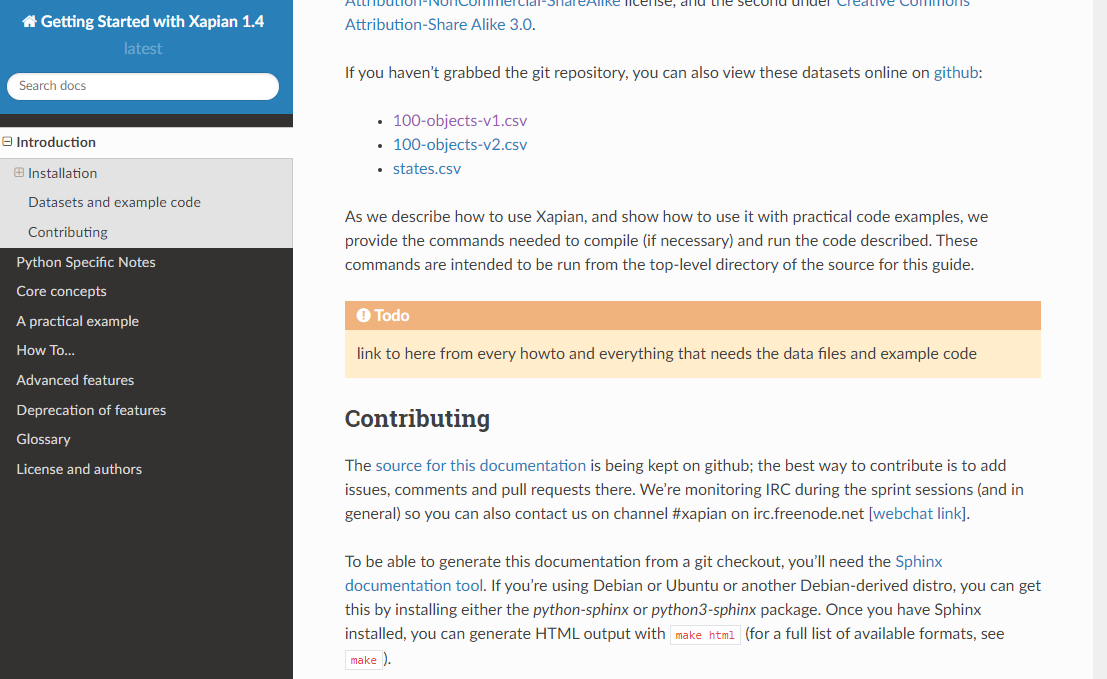
\includegraphics[width=1\linewidth]{images/xapian_doku.png}
	\caption{Screenshot von der Xapian Dokumentation}
	\label{img:xapianDoku}
\end{figure}

\subsection{Absetzen einer Anfrage und Integration in PHP}

Xapian besitzt keine REST-Schnittstelle. Daher wird der Befehl direkt auf mit PHP-Aufrufen gesendet. Dabei konnte aufgrund des Zeitkon­tin­gents die Remote Ausführung nicht getestet werden, da der Aufwand die PHP-Erweiterung auf Windows zu bauen, zu hoch war. Die Datei wurde deshalb direkt auf den Server ausgeführt, was bei der Laufzeit bedacht werden muss. 

Der Grund, warum eine eigene Zeile für den Buchstaben ausgewiesen werden muss, ist, dass Xapian generell nur Volltext ausweist. Es wurde zuerst versucht, mit Wildcards zu arbeiten, allerdings ergaben sich dabei dieselben Probleme, wie bei den anderen Suchmaschinen.

\begin{lstlisting}[language=php, frame=single, label={lst:XapPhpQuery}, 
	morekeywords={type,uninvertible,indexed,stored,field,multiValued, name}, caption=Skript zur Suche von Daten in Xapian,captionpos=b] 
// Require xapian.php and declare variables

$db = new XapianDatabase('db'); //Open Database

$queryParser = new XapianQueryParser();
//Set Prefix for Search
$queryParser->add_prefix("searchIndexLetter", "K"); 
$query = $queryParser->parse_query('S'); // Parse Query

//Loop for and time Results
// Use an Enquire object on the database to run the query
$enquire = new XapianEnquire($db);
$enquire->set_query($query);
$matches = $enquire->get_mset(0, 2147483647)->begin();
foreach ($matches as $pointer){
	$doc = $matches->get_document()->get_data();
	//$fields = json_decode($doc);
	$count++;
}
// Output Time for Run
//End Loop 
// Output Median Time
	
\end{lstlisting}

Nachdem die Abfrage die ersten hundert Male durchgelaufen war, war die Zeit mit 0.0044 Sekunden im Durchschnitt für die Ergebnisse sehr gering. Dies liegt daran, dass die Ergebnisse erstmal nur Pointer auf die kompletten Daten sind. 

Um nun alle Daten zu erhalten, muss nochmals ein gesonderter Befehl geschickt werden. Deswegen ist im Code ab Zeile 15 auch eine For-Schleife, welche die Datensätze für alle Pointer holt. Foreach verschiebt dabei automatisch den Pointer von den Ergebnissen. Wichtig ist, dass der Count ein Programmschritt ist, der theoretisch die Laufzeit erhöht und nicht für die normale Abfrage genutzt werden würde. Allerdings wurde diese Erhöhung hingenommen, um festzustellen, ob immer alle Ergebnisse korrekt geliefert werden.
Die auskommentierte Zeile würde das Objekt nun als Array mit Indices zurückgeben. 

Die Abfrage für das Abholen der Daten dauerte nun im Durchschnitt 0.22 Sekunden, was immer noch sehr schnell ist. Allerdings muss dabei bedacht werden, dass die Abfrage direkt auf dem Server lief, wodurch es keine Latenzzeit gab.


\section{Fazit}

TODO!
\chapter{Nutzung des Open Archives Initiative Protokolls für Metadaten}

Das Open Archives Initiative Protocol for Metadata Harvesting (OAI-PMH) ist ein Protokoll zum Austausch von Metadaten. Dabei werden Anfragen per GET oder POST-Request angefragt. Als Antwort erhält man im Folgenden ein XML-Dokument. So können die Metadaten mit bestimmten Facetten abgefragt werden (zum Beispiel Autor). Dabei geht es allerdings darum primär darum Änderungen weiterzugeben. So können durch dieses Protokoll neue Einträge oder Änderungen in der Datenbank weitergeben werden.
\cite{DeutscheNationalBibliothek.2019}

\section{OAI Harverester}

Ein OAI Harverester ist ein Programm, welches durchgehend einen Abgleich der Daten vollführt. Dabei lässt es sich die Änderungen mit einem List-Befehl von dem Server geben und gleicht diese danach mit der eigenen Struktur ab. Sollten dabei Unterschiede festgestellt werden, werden daraufhin die Änderungen auch beim Harverester eingefügt. So steht der Harverester immer mit dem Server auf einen Stand.
\cite{DeutscheNationalBibliothek.2019}

\section{Support der Enterprise Search Engines}

Bei den vorhin genannten Enterprise Search Engines gibt es keine mit nativen OAI Harverester Support. Es gibt die Möglichkeit für manche der Suchmaschinen ein solches Verhalten mithilfe von Plugins zu implementieren. Allerdings sind die meisten dieser Add-ons auch schon veraltet.

\section{Auswertung}

Durch eine fehlende Basisimplementierung des Protokolls in den einzelnen Suchmaschinen und der Möglichkeit eines direkten Zugriffs auf die Datenbank, sehe ich keinen Grund dieses Protokoll zu verwenden. Es müsste ein Server vor die Datenbank installiert werden und ein Harverester vor der ESE. Dies ist ein großer Mehraufwand, welcher bei diesem Anwendungsfall nicht notwendig ist. Sollte allerdings diese Suchmaschine ein übergreifendes System werden, kann darüber nachgedacht werden, die anderen Datenbanken per OAI-Harverester anzusprechen.
\chapter{Setup}

Dieses Kapitel behandelt die Installation und Ersteinrichtung der Suchmaschine. Die Installation erfolgt dabei über Docker mithilfe von Docker-Compose. Es werden 2 Elasticsearch-Instanzen, eine Kibana-Instanz und eine Logstash-Instanz aufgesetzt. Das fertig Setup soll dann wie folgt aussehen:

\begin{figure}
	\centering
	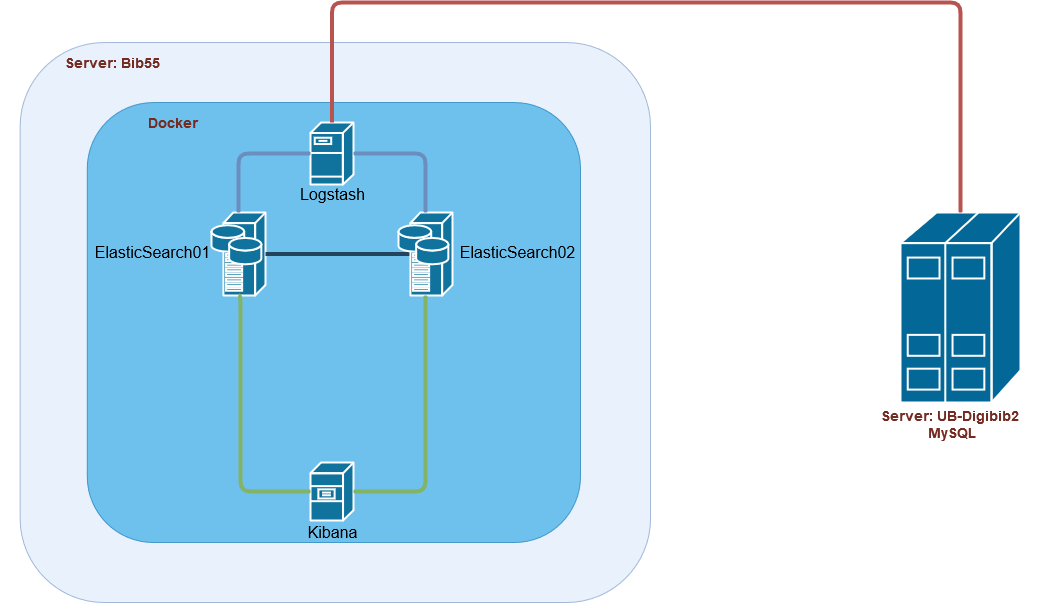
\includegraphics[width=1\linewidth]{images/docker_structure.png}
	\caption{Visualisierung des fertiges Docker-Netzwerkes}
	\label{img:dockerNetwork}
\end{figure}

Logstash sammelt die Daten von einem MySQL-Server und lädt sie in die Elasticsearch-Instanzen. Auch Kibana bekommt Zugriff auf beide Instanzen, um die Daten zu visualisieren und bei Serverausfällen frühzeitig zu warnen. Die beiden Elasticsearch-Instanzen halten sich dabei untereinander synchron. 

\section{Docker}

Docker ist eine Software zur Virtualisierung von Anwendungen. Dabei wird allerdings nicht, wie bei virtuellen Maschinen, die gesamte Hardware simuliert, sondern sie laufen im Kontext des Host-Betriebstystems.

Docker-Compose ist ein Tool, mit welchem es erleichtert wird, mehrere Docker-Container zu verwalten. Dafür werden in einer YAML-Datei\footnote{Kurz für YAML Ain't Markup Language, eine Konfigurationssprache \url{https://yaml.org/}} die gewünschten Docker-Container und Einstellungen, wie der Container-Name, eingetragen. Dies ist in Abbildung \ref{lst:es01} zu sehen. Mithilfe dieser Datei erstellt Docker-Compose dann die Container und Netzwerke automatisch.

\subsection{Rechteverwaltung in Docker}

Ein kurzer Exkurs zur Rechteverwaltung in Docker. Will ein Docker-Container auf dem Host-System schreiben, so nutzt dieser die Berechtigungen des Users innerhalb des Docker-Containers. Es kann allerdings passieren, dass die Nutzer-ID des Docker-Containers nicht der Nutzer-ID des Hosts entspricht. Werden nun Dateien im Hostsystem abgelegt, welche vom Container gelesen werden, muss dabei auf die Rechte geachtet werden. 

Elasticsearch verwendet die UID\footnote{Kurz für User identifier, Zahl zur Bestimmung eines Nutzers} und GID\footnote{Kurz für Group identifier, Zahl zur Bestimmung einer Nutzergruppe} von 1000. Auf dem Host-System ist dies jedoch ein anderer Nutzer. Das kann zu Problemen führen, da nun Dateien, welche für Elasticsearch gedacht sind, einem Nutzer, welcher nicht zu diesem Projekt gehört, gehören. Der Nutzer wurde nun auf eine andere UID gesetzt, um Verwirrung zu vermeiden. \cite{JarrodWeaver.2014}

\section{Elasticsearch}

Die beiden Elasticsearch-Instanzen bilden das Kernstück dieses Setups. Sie werden die Daten verwalten und sich untereinander synchronisieren. Dafür werden die beiden Instanzen als Cluster betrieben.

\begin{lstlisting}[language=YAML, frame=single, label={lst:es01}, caption=Auschnitt aus der Docker-Compose Datei,captionpos=b] 
es01:
image: docker.elastic.co/elasticsearch/elasticsearch:7.5.1
container_name: es01
environment:
	- "ES_JAVA_OPTS=-Xms4g -Xmx4g"
ulimits:
	memlock: -1
volumes:
	- /srv/elk/elasticSearch01/:/usr/share/elasticsearch/data
	- /srv/elk/config/elasticsearch.yml:
		/usr/share/elasticsearch/config/elasticsearch.yml
ports:
	- 9200:9200
networks:
	- elastic
\end{lstlisting}

Das Listing \ref{lst:es01} zeigt einen Auschnitt aus der Docker-Compose, in welchem die ersten Einstellungen getroffen werden.

Für die beiden Elasticsearch-Instanzen wird der Java-Speicher auf 4 Gigabyte gesetzt. Dies errechnet sich dadurch, dass der Server 16 Gigabyte RAM besitzt und die Elasticsearch-Instanzen nicht mehr als 50 \% des gesamten RAMs verwenden sollten. \cite{ElasticsearchB.V..12172019}

Der ulimits Befehl hebt die Begrenzung des Memory-Locks auf, damit Elasticsearch korrekt arbeiten kann. Dadurch wird der RAM von Elasticsearch nicht in den SWAP-Speicher\footnote{Speicher auf der Festplatte, welcher von Linux genutzt wird, falls der RAM voll ist.} gelegt. Dies würde die Leistung von der Suchmaschine stark beinträchtigen.

Als Volumes ist zum einen die oben genannte YAML-Datei angegeben und zum anderen wird der Datenordner gemountet. Dies dient dazu, dass, falls der Container zerstört wird, die indexierten Daten trotzdem weiterhin auf dem Host-System verbleiben.

Der Port wird zum Host-System durchgereicht, damit das System auch von außerhalb des Docker-Netwerkes zu erreichen ist. Dabei ist das System trotz blockierter UFW\footnote{UFW ist die uncomplicated Firewall, eine Firewall-Software für Linux} zu erreichen. Dies liegt daran, dass die Docker-Container in der Standardeinstellung die UFW ignorieren.

In der Elasticsearch-Konfigurationsdatei werden nun die Einstellungen, die speziell für das Elasticsearch-System relevant sind, verwaltet: 

\begin{lstlisting}[language=YAML, frame=single, label={lst:es01-yml}, caption=Auschnitt aus der Konfigurationsdatei von Elasticsearch,captionpos=b] 
cluster.name: dietrich-online-cluster
node.name: es01
bootstrap.memory_lock: true
network.host: 0.0.0.0
discovery.seed_hosts: ["es02"]
cluster.initial_master_nodes: ["es01", "es02"]
\end{lstlisting}

Darin wird zuerst der Cluster-Name definiert. Dieser dient dazu, dass die Server wissen, dass sie dieselben Daten betreuen. 
Danach wird der Name des Servers vergeben, welcher der Identifizierung dient.

Das Memory-Lock Setting dient dazu, dass die Anwendung verhindert, dass sie in den SWAP gelegt wird.

Der Network Host wird hier auf alle Interfaces der Maschine gesetzt, damit sich alle Systeme innerhalb der Docker-Netzwerkes finden können.

Das Seed-Host Setting sagt aus, an welchen Nodes\footnote{Hier: Elasticsearch-Instanzen} die Daten synchronisiert werden sollen.

Der letzte Eintrag dient dazu, dass bei der ersten Synchronisation das System weiß, welche Nodes alle Daten enthalten, also mit welchen Server sich synchronisiert werden soll. Da hier beide Systeme beim ersten Start noch keine Daten besitzen, sind alle Nodes zu beginn Master. \cite{ElasticsearchB.V..13.2.2020}


\section{Kibana}

Die Grundkonfiguration von Kibana ist einfacher als die Konfiguration von Elasticsearch. Es muss nur die YAML-Datei in den Container geladen werden und der Port 5601 nach außen durchgereicht werden.

In der Konfigurationsdatei werden nun die Einstellungen für Kibana gesetzt. Darunter fällt der oben genannte Port, der Server-Host, in diesem Fall auch 0.0.0.0, und die Elasticsearch-Hosts. Dabei werden alle Server-Instanzen mitgegeben, auf denen Kibana arbeiten soll. \cite{ElasticsearchB.V..12.2.2020}

\section{Logstash}

Für die Grundkonfiguration von Logstash muss, wie schon im Ersteindruck, der Treiber in die Core-Bibliothek gelegt werden. Zudem werden die Konfigurationsdateien für die Pipelines gemountet.

In der Konfigurationsdatei für Logstash wird dann der Name, die Pipeline.id und die Pipeline-Worker festgelegt. Die Pipeline-Worker sind die Threads, in denen eine der konfigurierten Pipelines abgearbeitet wird. Generell sollte die Anzahl der Cores auch die maximale Anzahl der Worker sein. \cite{ElasticsearchB.V..12.2.2020b}


\section{X-Security}

X-Security nennt sich das Paket, mit den Sicherheitseinstellungen für den ELK-Stack. In diesem Schritt wird der komplette Datenverkehr zwischen den einzelnen Komponenten, sowie vom Endnutzer zum Server mit SSL verschlüsselt. 

Dazu werden zuerst die Zertifikate generiert. Dafür bietet Elasticsearch ein Tool an, welches eine Zertifikats-Autorität (CA)\footnote{Mithilfe einer CA kann sich ein Klient gegenüber des Servers ausweisen und umgekehrt.} und die einzelnen Zertifikate mit Private- und Public-Key generiert. Allerdings werden diese standardmäßig im PKCS 12-Format abgespeichert. Dieses ist ein Container-Format, welches die Schlüssel und die CA zusammen verpackt. Jedoch benötigt Kibana zum Beispiel nur die Autorität als einzelnes Zertifikat und nicht den Container.

Normalerweise gibt es eine Möglichkeit, dieses Zertifikat aus der PK12-Datei zu entpacken, jedoch gab es hierbei Probleme, da OpenSSL, das Tool welches zum Entpacken verwendet wird, die CA nicht richtig entpacken kann. \cite{nerophon.2018}

Die Lösung dieses Problems war es, schon bei der Zertifikaterstellung eine Option mitzugeben, dass die Zertifikate nicht verpackt werden sollen. 

Um nun alle Zertifikate gleichzeitig zu generieren, kann eine YAML-Datei mitgegeben werden. In dieser werden dann die Details für die Zertifikate, wie zum Beispiel DNS-Name und IP des Servers, mitgegeben. In diesem Fall wurde nur der DNS-Name angegeben:
\newpage

\begin{lstlisting}[language=YAML, frame=single, label={lst:certs-yml}, caption=Auschnitt aus der Konfigurationsdatei für die Zertifikatgenerierung,captionpos=b] 
instances:
- name: 'es01'
	dns: [ 'es01', 'bib55', 'bib55.uni-trier.de' ]
[...]
\end{lstlisting}

Damit diese Zertifikate auch genutzt werden können, muss jeder Container das zugehörige Zertifikat einbinden. Zudem wurden in den dazugehörigen Konfigurationsdateien die jeweiligen Optionen zur Nutzung der CA und Private-Keys gesetzt.

Zusätzlich zu den Zertifikaten muss noch eine Passwort-Authentifikation eingebaut werden. Dazu kann auf den Elasticsearch-Containern ein Befehl zur Erstellung der Systempasswörter aufgerufen werden. Dadurch werden alle Benutzer, welche die einzelnen Systeme wie Logstash oder Kibana zum Funktionieren brauchen, generiert.

Auch diese müssen in den Konfigurationsdateien vermerkt werden. Weitere Nutzer können von nun an per API oder Kibana erstellt werden. Die Verteilung der Rechte ist hierbei rollenbasiert. Es wird zuerst eine Rolle erstellt, welche die gewünschten Rechte enthält, die daraufhin an den Nutzer weitergegeben wird. Dabei können die Rollen sehr spezifisch angepasst werden. Es können einzelne Systemfunktionen, wie die Erstellung von Snapshots, spezifisch freigegeben werden. Hierbei sollte sich an das Minimalprinzip gehalten werden, also nur genau die Rechte vergeben werden, welche der Nutzer auch benötigt. Zusätzliche Rechte werden dem Nutzer dabei verwehrt. \cite{ElasticsearchB.V..13.2.2020}

Um nun eine Abfrage gegen das Elasticsearch-System zu stellen, muss zum einen eine BasicAuth, sowie die CA mitgegeben werden:

\begin{lstlisting}[language=BASH, frame=single, label={lst:curlQuery}, caption=Curl-Abfrage an das Elasticsearch-System,captionpos=b] 
curl https://bib55:9200 --cacert ca.crt -uuser:pass
\end{lstlisting}

Damit Logstash wieder Daten an Elasticsearch senden kann, wird ein Nutzer erstellt, welcher nur auf Indices mit dem Präfix dietrich\_ Zugriff erhält. Die Erstellung von diesem Nutzer erfolgte dabei über die Benutzer-Oberfläche von Kibana: 

\begin{figure}
	\centering
	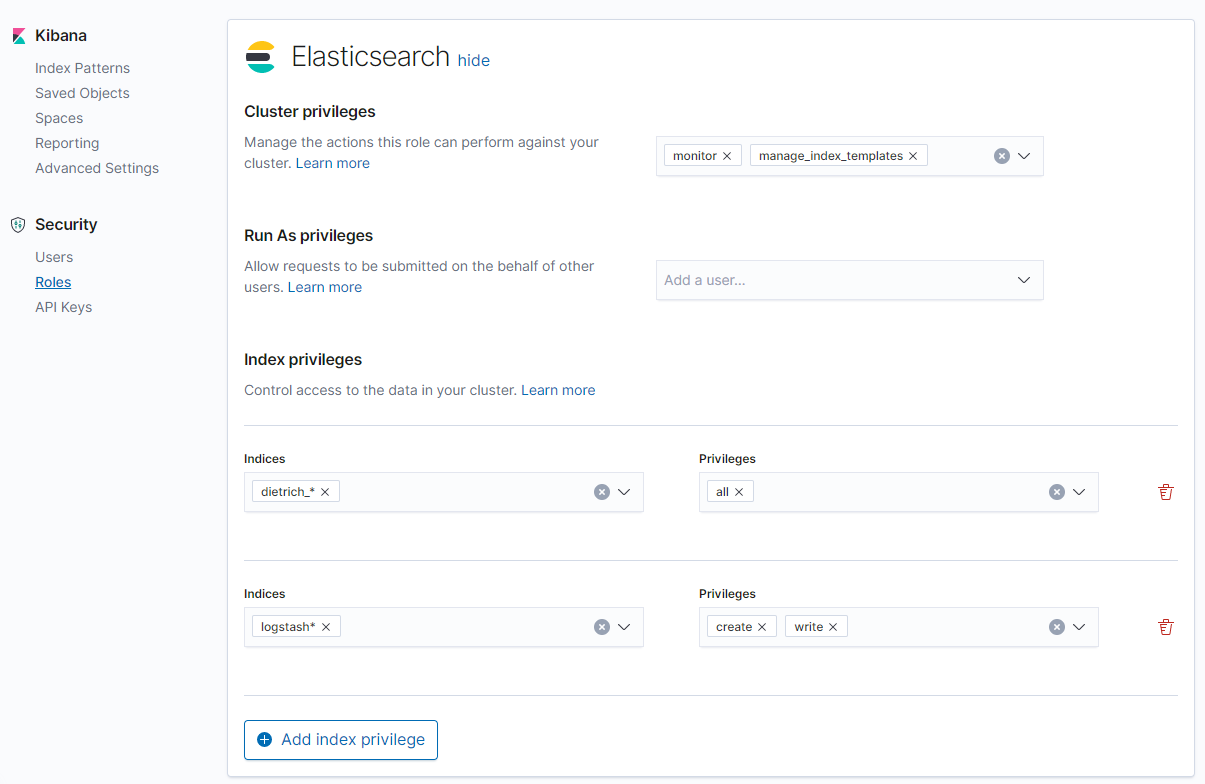
\includegraphics[width=1\linewidth]{images/setup/kibana_roles.png}
	\caption{Seite zu Erstellung von Rechte-Rollen}
	\label{img:kibanaRoles}
\end{figure}
\chapter{Implementation in das Dietrich Projekt}

In diesem Kapitel wird die Implementation ins Dietrich-Projekt genauer erläutert.

\section{Vorbereitung}

Zuerst muss der ElasticSearch Client in der Docker-Compose hinzugefügt werden. Die folgenden Vergleiche wurden in einem Docker-System gemacht mit Remote-Verbindung zur Datenbank und ElasticSearch. 

\subsection{ElasticSearch}

Zuerst soll der Lemma-Query der auch schon zum Testen in finaler Fassung in das Dietrich-Online Projekt integriert werden.

Zu Beginn muss dafür ein API-Key generiert werden, um Zugriff auf die benötigten Indices zu erhalten. Dies kann entweder über die Entwicklerkonsole oder eine Curl Abfrage geschehen \ref{lst:elaApi}. Mit diesen Key und der CA ist es nun möglich Anfragen an das ElasticSearch zu stellen.

\begin{lstlisting}[language=XML, frame=single, label={lst:elaApi}] 
    POST /_security/api_key
    {
      "name": "dietrich-webiste",
      "role_descriptors": { 
        "role-a": {
          "cluster": ["all"],
          "index": [
            {
              "names": ["dietrich_*"],
              "privileges": ["read"]
            }
          ]
        }
      }
    }
\end{lstlisting}


\subsection{Einbindung in Dietrich-Online}

Die Einbindung in das Dietrich-Online Projekt lief über KACKE

\subsubsection{Indexierung}

Da nun nicht einfach nur die Daten in das System eingepflegt werden, wurde diesmal auf die Indexierung mehr Wert gelegt. Damit Arrays ordentlich abgebildet werden, musste in der Logstash Datei Daten richtig aggregiert werden. 


//TODO RUBY


\subsection{Vergleich}

Für den Vergleich wurde zum einen 100 mal die Geschwindigkeit getestet, um die Daten in weiterverarbeitbarer Form zu bekommen.
Dafür wurden die beiden Methodenaufrufe, welche die Query generieren und ausführen, mit einem Timer umhüllt. Die erste Methode holt sich dabei alle Ids von den benötigten Lemmata und die zweite baut alle Daten zusammen, welche zur Anzeige benötigt werden. Als Framework wird für die Querys Doctrine verwendet, was sich auch um die Datenerhaltung kümmert.

\begin{lstlisting}[language=PHP, frame=single, label={lst:vglDb}] 
  ini_set('max_execution_time', 3000);

  $timeAcc = 0;
  for ($i = 0; $i < 100; $i++) {
    $time_start = microtime(true);

    $lemmas   = $this->findLemmaByCharacter($character, $filter);
    $results  = $this->findLemmaById($lemmas);

    $time_end = microtime(true);
    $time     = $time_end - $time_start;
    $timeAcc     += $time;
    echo $time.'<br/>';
  }
  
  echo 'Combined Time'.$timeAcc / 100 .'<br/>';
  die;
\end{lstlisting}

Bei ElasticSearch sieht der Query ähnlich aus. Allerdings wird hierbei ein Array generiert und es wird nur eine Abfrage gestellt. 

Bei dem Vergleich kamen die folgenden Durchschnittswerte zustande:
\begin{table} %[hbtp]
	\centering
		\begin{tabular}{l | l }
		    \textbf{System} & \textbf{Zeit} \\
        \hline
        MariaDB + Doctrine & 3.49 \\
        ElasticSearch      & 1.45  \\
		\end{tabular}
    \caption{Vergleich der Laufzeit zur Abfrage aller Daten für Buchstabe S der Lemma-Administration (15.846 Einträge)}
    \label{vlgTimeDBvsEla}
\end{table}


\begin{figure}
	\centering
	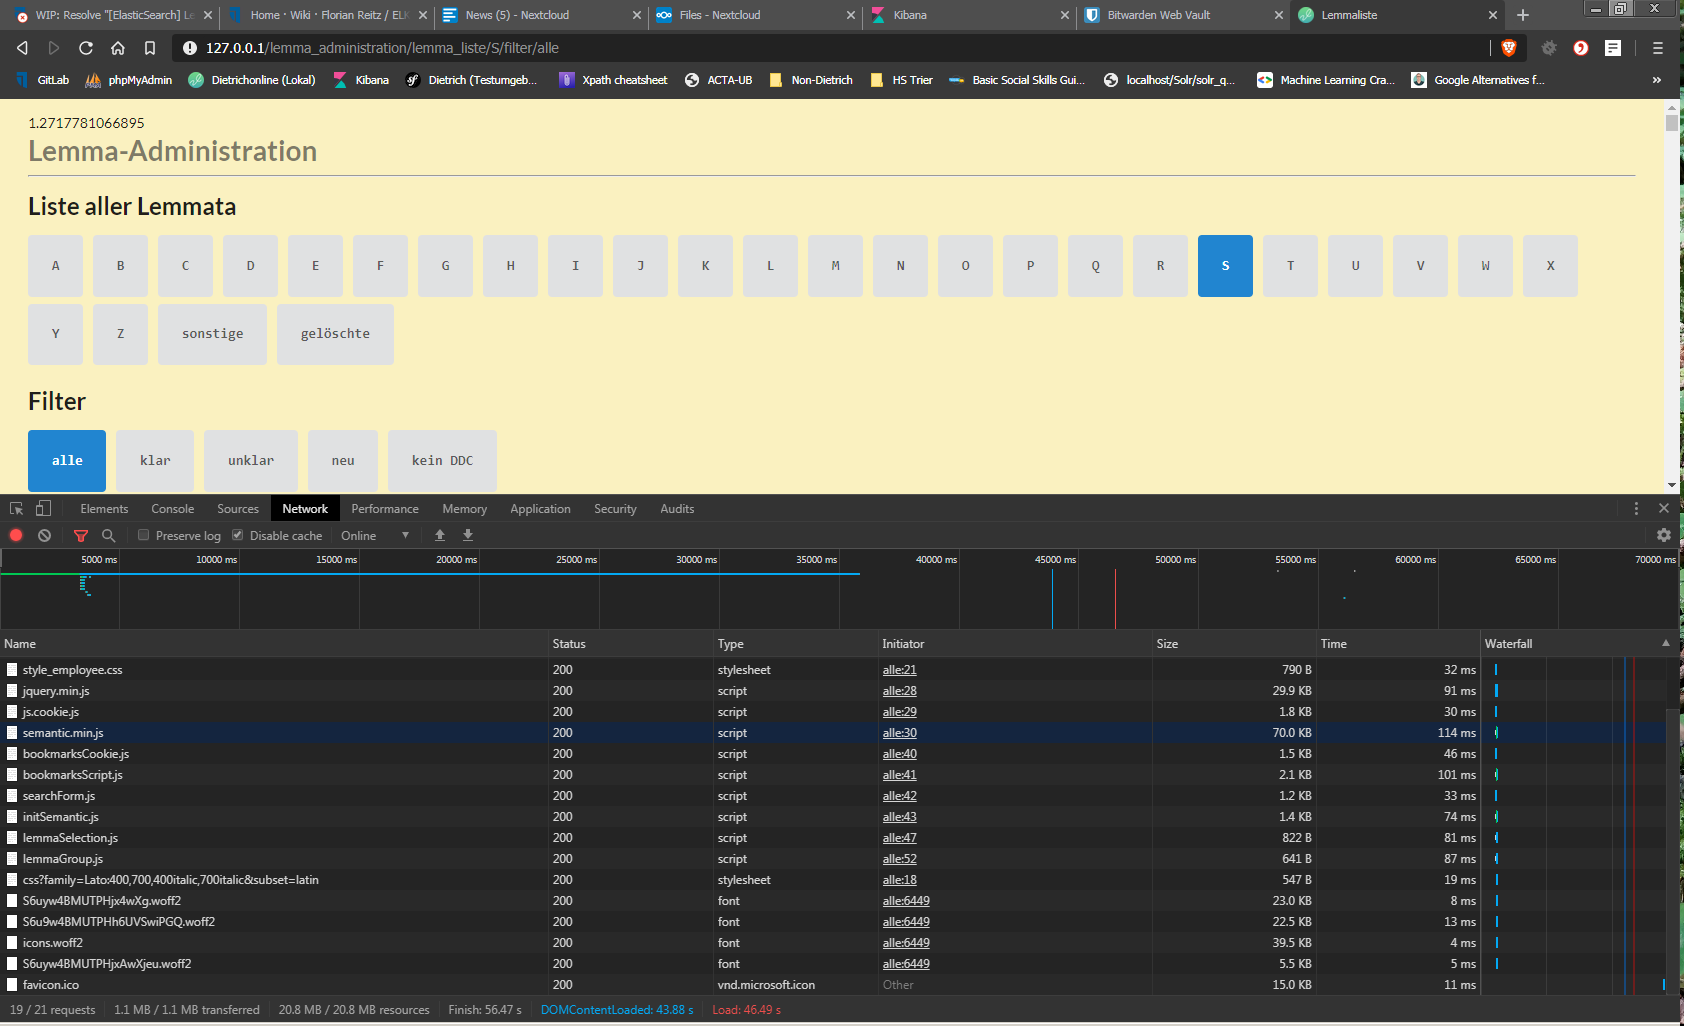
\includegraphics[width=1\linewidth]{images/setup/query/time_prod_ela.png}
	\caption{Seite zu Erstellung von Rechte-Rollen}
	\label{img:timeProdEla}
\end{figure}

\begin{figure}
	\centering
	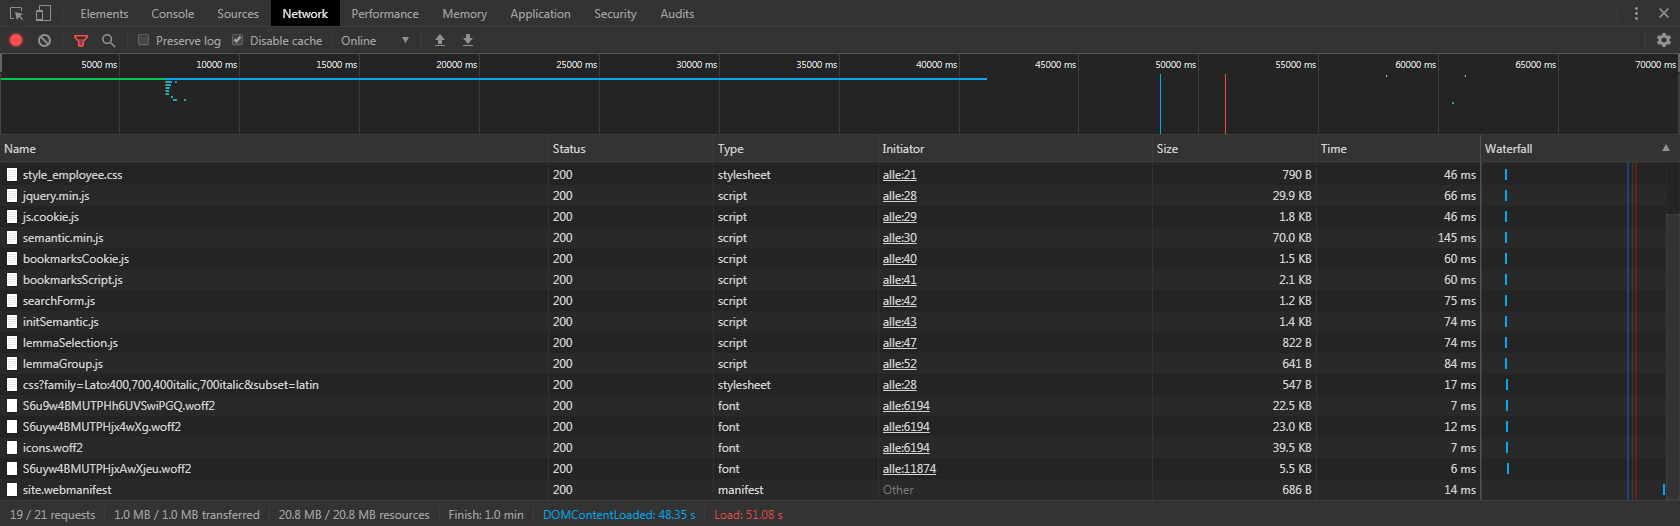
\includegraphics[width=1\linewidth]{images/setup/query/time_prod_db.png}
	\caption{Seite zu Erstellung von Rechte-Rollen}
	\label{img:timeProdDb}
\end{figure}



\begin{lstlisting}[language=PHP, frame=single, label={lst:queryEla}] 

  //Create Client with basic Params

  $mustNotQueries = [];
  $filters        = [];
  $mustQueries    = [];

  if ($character === LemmaEntity::NOT_A_TO_Z_CHARACTER) {
      $mustQueries[] = ['regexp' => ['bezeichnung.keyword' => 
        ['value' => '@&~(^[a-zA-Z].+)', 'flags' => 'ALL']]];
        
      $filters[]     = ['term' => ['ist_geloescht' => false]];
  } elseif ($character === LemmaEntity::DELETED) {
      $filters[] = ['term' => ['ist_geloescht' => true]];
  } else {
      $mustQueries = ['prefix' => ['bezeichnung.keyword' => "$character"]];
      $filters[]   = ['term' => ['ist_geloescht' => false]];
  }

  switch ($filter) {
      case self::STATUS_FILTER_KLAR:
          $filters[] = ['term' => ['bstatusbezeichnung' => 'klar']];
          break;
      //[Other Filters]
  }

  $params['body']['query']['bool']['must']     = $mustQueries;
  $params['body']['query']['bool']['must_not'] = $mustNotQueries;
  $params['body']['query']['bool']['filter']   = $filters;

  return $client->search($params)['hits']['hits'];

\end{lstlisting}

DEr query hat must, should and shouldnt

Anders als bei der Test Query \ref{lst:phpElastic} wurde bei dieser Query der Filter Prefix verwendet. Dies liegt daran, dass Praefix schneller agiert als ein Wildcard Query.
\chapter{FrontEnd}

\chapter{Zusammenfassung und Ausblick}

Diese Bachelorarbeit hat sich ausführlich mit Enterprise-Suchmaschinen auseinandergesetzt, diese Verglichen und letztendlich eine in das DietrichOnline-Projekt implementiert. Das Ziel dabei war es eine geeignete Suchmaschine für dieses Projekt zu finden und implementieren.  

Im ersten Schritt wurden diverse Suchmaschinen erstmal nach einer Anforderungsliste verglichen. Dafür wurde eine Tabelle erstellt, welche alle Suchmaschinen anhand der gefundenen Funktionen verglichen. Mithilfe dieser Basis wurden vier Suchmaschinen für den genaueren Vergleich herausgesucht.

Für den genaueren Vergleich wurden diese Suchmaschinen nacheinander aufgesetzt und einige Dokumente indexiert. Dabei musste die Suchmaschine selbständig die Daten aus der Datenbank laden und indexieren. Zudem wurde auch die Benutzerfreundlichkeit untersucht. Dafür wurde die Oberfläche, insofern eine vorhanden war, und die Dokumentation bewertet. Zum Schluss wurde daraufhin eine Suchmaschine ausgewählt, welche in das DietrichOnline-Projekt implementiert werden sollte. Dabei war es aufgrund der Zeit leider nicht möglich einen korrekten wissenschaftlichen Vergleich zu erstellen. Es wurde lediglich ein Ersteindruck gewonnen.

Als Nächstes wurde über die Möglichkeit nachgedacht einen OAI Harverester vor die Datenbank zu stellen, um eine normierte Schnittstelle zwischen der Datenbank und Suchmaschine herzustellen. Nach einer kurzen Analyse wurde diese Methodik allerdings verworfen, da ein direkter Zugriff auf die Datenbank möglich ist und somit der Vorgang um an die zu indexierenden Daten zu kommen nur komplizierter gestaltet wird. Diese Funktion könnte allerdings für Datenbanken ohne direkten Zugriff interessant sein. 

Nachdem nun eine Suchmaschine ausgewählt wurde, ging es nun darum diese ordentlich aufzusetzen. Dabei wurde in dieser Arbeit Docker-Compose verwendet. Die Kommunikation zwischen den einzelnen virtuellen Containern wurde hierbei mit selbst generierten Zertifikaten verschlüsselt. Dabei kam es zu einigen Problemen mit der Generierung und Verwendung der Zertifikate, weshalb darüber nachgedacht werden sollte, ob die Verschlüsselung innerhalb des Systems zielführend ist, insofern das System weiterhin auf einen Server laufen soll. 

Im letzten Schritt wurde nun noch eine prototypische Implementierung in das Projekt vorgenommen. Dafür wurde ein Index mit allen für die Suche wichtigen Daten aufgebaut. Um die Größe des Indexes zu minimieren wurde für alle Felder ein vorheriges Mapping vorgenommen. Zudem wurden extra Felder für eine Auto-Vervollständigungsfunktion indexiert. Mithilfe dieses Indexes wurde die Suche für die Nutzer verbessert. Es werden nun mehr verschiedene Sucharten unterstützt. Auch ist es nun möglich mehr als 1001 Ergebnisse zu erhalten. Dies war vorher eine durch die Datenbank auferlegte Grenze. Um zu zeigen, was die Suchmaschine sonst noch für Funktionen unterstützt wurde zudem eine Funktion eingebaut, die die zehn Autoren auflistet, welche die meisten Artikel in der aktuellen Suche geschrieben haben. 

Es wurde für einen Vergleich noch ein Index über alle Lemmata aufgebaut. Dieser ist der aktuell am langsamsten ladende Teil des Projekts. Mit dem Wechsel auf Elasticsearch ist es so gelungen die Laufzeit von dieser Abfrage, um 50 \% zu verringern. 

Zur Implementierung wurde der offizielle Klient von Elasticsearch verwendet, welcher auf einer sehr niedrigen Ebene arbeitet. Es gibt auch Klienten, welche das Level ein wenig mehr abstrahieren und so eine angenehmere Erfahrung bieten, allerdings diese alle nicht offiziell unterstützt. Daher habe ich mich in dieser Arbeit auf den Klienten von Elasticsearch fokussiert. 

Sobald die Suchmaschine in das Projekt eingegliedert ist, können viele weitere Probleme des Projektes gelöst werden. So können zum Beispiel Synonymlisten für Autoren geführt werden, um die verschiedenen Schreibweisen bestimmter Autoren auszugleichen. Auch ist es mit der Suchmaschine möglich dem DDC-Baum, welcher schon seit langer Zeit implementiert werden sollte, leichter einzubauen. Zudem bietet Elasticsearch Funktionen zur Autokorrektur, welche die Sucherfahrung positiv bereichern können. Und für die Entwickler nimmt Elasticsearch einiges an Problemen mit der Datenbank ab. Aktuell werden viele Felder mithilfe von Triggern und Funktionen erstellt. Diese Trigger können nun auf Logstash übertragen werden, um so die Datenbank zu entlasten.

Damit nicht bei jeder Anfrage eine Zertifikats-Autorität mit gereicht werden muss, kann auch noch ein sogenannter Reverse Proxy vor die Elasticsearch Instanz gesetzt werden, welcher daraufhin Zertifikate mithilfe von LetsEncrypt generiert.
% ...
%--------------------------------------------------------------------------
\backmatter                        		% Anhang
%-------------------------------------------------------------------------
\bibliographystyle{IEEEtranHS.bst}			% Literaturverzeichnis
\bibliography{literatur}     			% BibTeX-File literatur.bib
%--------------------------------------------------------------------------
\printindex 							% Index (optional)
%--------------------------------------------------------------------------
\begin{appendix}						% Anhänge sind i.d.R. optional
   \chapter{Glossar}

\abbreviation{ESE}{Enterprise Search Engine}
\abbreviation{Facetten}{Filter in Bibliothekarssprache}
\abbreviation{OAI}{Open Archives Initiative}
\abbreviation{OCR}{Optical Character Recognition}
			% Glossar   
   \chapter{Erklärung der Kandidatin / des Kandidaten}

\begin{description}[$\Box$~]
\item[$\Box$] Die Arbeit habe ich selbstständig verfasst und keine anderen als die angegebenen Quellen und Hilfsmittel verwendet.\\
\end{description}

\vspace{2cm}

\begin{minipage}[t]{3cm}
\rule{3cm}{0.5pt}
Datum
\end{minipage}
\hfill
\begin{minipage}[t]{9cm}
\rule{9cm}{0.5pt}
Unterschrift der Kandidatin / des Kandidaten
\end{minipage}	% Selbstständigkeitserklärung
\end{appendix}

\end{document}
